% ══════════════════════════════════════════════════════════════════
% ETRIZAÇÃO COMPUTACIONAL EM DOENÇAS PRIÔNICAS — EDIÇÃO DE LEITURA
% Gerado por scripts/build_reader_edition.py a partir do mestre-gated
% (tese_unificada.md · guardian 0/0 · AST 10/10). NÃO editar à mão.
% Numeração: só LaTeX · zero tags no corpo · provenance no apêndice.
% ══════════════════════════════════════════════════════════════════
\documentclass[12pt,a4paper,oneside]{report}
\usepackage[brazil]{babel}\usepackage{fontspec}\setmainfont{TeX Gyre Termes}
\usepackage[a4paper,top=3cm,bottom=2cm,left=3cm,right=2cm]{geometry}
\usepackage{amsmath,amssymb,graphicx,booktabs,longtable,microtype}
\usepackage{array,calc,xcolor}
\providecommand{\tightlist}{\setlength{\itemsep}{2pt}\setlength{\parskip}{0pt}}
\usepackage{caption}\captionsetup{font=small,labelfont=bf,skip=6pt}
\usepackage[htbp]{float}
\usepackage{fancyhdr}\pagestyle{fancy}\fancyhf{}
\fancyhead[L]{\small\itshape Etrização computacional em doenças priônicas}
\fancyhead[R]{\small\thepage}\renewcommand{\headrulewidth}{0.3pt}\setlength{\headheight}{15pt}
\raggedbottom
\providecommand{\pandocbounded}[1]{#1}
\usepackage{newunicodechar}
\newunicodechar{↔}{\ensuremath{\leftrightarrow}}\newunicodechar{∂}{\ensuremath{\partial}}
\newunicodechar{∇}{\ensuremath{\nabla}}\newunicodechar{✅}{\ensuremath{\checkmark}}
\newunicodechar{⚠}{\textbf{!}}\newunicodechar{⁻}{\ensuremath{^{-}}}\newunicodechar{⇒}{\ensuremath{\Rightarrow}}\newunicodechar{→}{\ensuremath{\to}}\newunicodechar{↦}{\ensuremath{\mapsto}}\newunicodechar{∝}{\ensuremath{\propto}}\newunicodechar{≈}{\ensuremath{\approx}}\newunicodechar{≡}{\ensuremath{\equiv}}\newunicodechar{∴}{\therefore}\newunicodechar{️}{}\newunicodechar{〔}{}\newunicodechar{〕}{}
\usepackage[colorlinks=true,linkcolor=black,citecolor=black,urlcolor=blue,
pdftitle={Etrização Computacional em Doenças Priônicas: Aplicada à Plataforma Terapêutica PrP-V127},
pdfauthor={Camilla N.}]{hyperref}
\title{Etrização Computacional em Doenças Priônicas:\\Aplicada à Plataforma Terapêutica PrP-V127}
\author{Camilla N.}\date{2026}
\begin{document}
\maketitle
\chapter*{Resumo}\label{resumo}

\textbf{Introdução.} Doenças priônicas são 100\% fatais e seis
candidatos clínicos fracassaram sem modelo quantitativo de entrega. A
Parte 1 construiu, por auditoria sistemática, física de transporte,
calibração bayesiana e simulação humanizada, uma plataforma de contenção
terapêutica (PrP-V127) com limiar adimensional θ*=0,333 --- executada,
aprovada e reproduzida em dois ambientes computacionais.
\textbf{Objetivo.} Esta tese unificada formaliza e realiza a
continuidade: (i) nomeia e formaliza o método que a sustenta --- a
etrização computacional, passos P0--P6; (ii) estabelece a Base de
Validade com linhagem completa de cada dado; (iii) declara a tese em
forma experimental análoga; (iv) entrega os resultados como os achados
{[}SIM{]} executados --- agora incluindo a validação multi-espécie de θ*
(Parte 3) e a primeira dose calculada do braço discriminador A6 com
incerteza propagada; e (v) documenta, como método replicável, a seleção
futura de parceiros sem executá-la. \textbf{Método.} Etrização P0--P6
sobre base E-registrada (58 fontes verificadas), motores determinísticos
auto-testados (conservação de massa 100\%; erro de Thiele 0,5\%),
colheita sob critérios pré-declarados, prognósticos travados por release
antes de qualquer medição, estimador θ\_obs calibrado por simulação,
guardião recursivo R0--R3 em dois perfis de superfície, cadeia
dimensional de dose κ→µM→µg/depósito em banda GUM Tipo-B (âncora
ilustrativa, fechada pelo braço A6) com critérios de aceitação
pré-registrados. \textbf{Resultados.} Limiar θ*=0,333; três regras de
design; Cenário B multi-espécie (θ* 0,333--0,400 centrais; razão 1,20)
com regra de titulação κ↔Kt; banda de dose A6 no degrau humano: 0,0--2,6
µg de V127ΔGPI por depósito (pior caso κ=8: 0,2--10,3 µg; redose ≤7 d;
MW 22,83 kDa das sequências próprias) --- a largura da banda ≈53× é o
achado, dominada pelo proxy de Kd, até o braço G0-A6 fechá-la; registro
de 60 claims, 58 fontes, 65 fatos numéricos com validação por máquina.
\textbf{Conclusão.} A tese está realizada --- \textbf{e é uma
etrização}: entregue, rotulada, auditável --- nos termos da etrização:
continuar pesquisa por simulação parametrizada sem substituir o
laboratório --- se dados reais futuros forem análogos aos simulados, os
passos seguintes já estarão avançados (antecipação bancada).

\textbf{Palavras-chave:} etrização; príons; simulação computacional;
etrização computacional; PrP-V127; doença de Creutzfeldt-Jakob;
metodologia de pesquisa; in-silico; dose-band.

\begin{quote}
\mbox{}%
\section{\texorpdfstring{NOTA À LEITURA --- SOBRE O TERMO
\emph{ETRIZAÇÃO}}{NOTA À LEITURA --- SOBRE O TERMO ETRIZAÇÃO}}\label{nota-uxe0-leitura-sobre-o-termo-etrizauxe7uxe3o}

Este documento introduz o termo \textbf{etrização} como neologismo
científico composicional intencional. O radical \emph{etr-} evoca, por
extração morfológica deliberada (não derivação etimológica), a evolução
\emph{essere→estre→être} da raiz indo-europeia *es- (`ser') --- o
\textbf{potencial de vir a ser} --- e o \emph{atrium} latino --- a
\textbf{antecâmara} entre o virtual e o real. \textbf{Etrização} nomeia
o estado do conhecimento que esta tese produz e entrega: um sistema
operacionalizado computacionalmente a partir de dados reais publicados,
estruturalmente robusto e preditivamente informativo, \textbf{ainda não
validado empiricamente} --- e por isso mesmo capaz de fundamentar as
pesquisas subsequentes que o atualizarão. Como o `átomo' nomeou antes da
prova um objeto que fundou ciência, `etrização' nomeia o processo que
produz objetos-conceito operacionais na saúde. O método que a produz,
com seus passos e garantias, é a ACP (Cap. Métodos); a operação técnica
central é a parametrização com proveniência. Cinco critérios distinguem
uma etrização de mera simulação --- cadeia de dados explícita,
transposição justificada, incerteza quantificada, escopo delimitado,
transição condicionada --- \textbf{todos cumpridos e auditáveis nesta
tese}. E, como mandato: toda a simulação aqui se alimenta exclusivamente
de fatos e dados amplamente divulgados na literatura publicada.

\textbf{Protocolo metodológico de leitura (como auditar o que vai ler).}
(i) Todo dado carrega rótulo de tier:
\textbf{{[}SIM{]}/{[}ORGANOID{]}/{[}MOUSE{]}/{[}HUMAN{]}} --- toda cifra
desta edição é {[}SIM{]}: simulação parametrizada sobre fontes reais,
nunca medida; (ii) toda afirmação-numérica amarra a claim (C-ID) e
referência (E-ID → lista ABNT ao final); a concordância integral está
tabelada; (iii) as predições centrais estão travadas por release público
(v1.0) desde antes de qualquer resultado --- comparações jamais
reescrevem o passado (anti-hindsight); (iv) o documento foi verificado
por revisão hostil de máquina (guardião R0--R3) e pela bateria AST 9/9
--- reproduzível com \texttt{python3\ experiments/ast\_check.py}; (v) a
simulação \textbf{não substitui} o laboratório: o caminho obrigatório
até a sociedade está declarado no Cap. 9 (próximas abordagens).
\end{quote}

\tableofcontents
\listoffigures
\listoftables
\section{LISTA DE SIGLAS}\label{lista-de-siglas}

ETRIZAÇÃO/etrização computacional --- o método nomeado desta tese
(neologismo composicional; en: Computational Etrization) · θ --- fração
de replicação remanescente no pico secretor, θ≡(1+κ·c\_pico)⁻¹ ·
\textbf{θ*} --- θ no limiar de contenção (predição travada v1.0: 0,333)
· \textbf{θ\_obs} --- estimador que mede o análogo de θ* num gradiente ·
\textbf{κ} --- força de capping (a ``dose'' do agente; âncora κ↔µM em
banda GUM via Kd aparente --- âncora ilustrativa, fechada pelo braço A6)
· \textbf{κ\_req} --- κ requerido para contenção numa banda-Kt dada
(regra de titulação) · \textbf{Kt} --- classe de taxas de
autocatálise/templating (a única que governa contenção e relógio ---
F-43) · \textbf{banda-Kt} --- faixa de cinética do hospedeiro (humano:
\{0,5·1·2\}) · \textbf{MW} --- massa molecular (PrP maduro humano: 22,83
kDa, computada das sequências próprias) · \textbf{Damköhler} --- razão
velocidade-de-reação/velocidade-de-difusão · \textbf{PrP\^{}C /
PrP\^{}Sc} --- proteína prion celular / forma scrapie · G0-sim/G0-wet
--- gates computacional/organoide · T1/T2/T3 --- níveis de aceitação ·
{[}SIM{]}/{[}ORGANOID{]}/{[}MOUSE{]}/{[}HUMAN{]} --- tiers de dado · SLR
--- revisão sistemática de literatura · PPS --- pentosan-polissulfato ·
CrI --- intervalo de credibilidade · ADR --- advecção--difusão--reação ·
ECS --- espaço extracelular · RT-QuIC --- ensaio de sementeamento in
vitro · DN --- dominante-negativo · GUM --- Guia para a Expressão da
Incerteza de Medição (Tipo-B: incerteza avaliada por julgamento/fonte,
não por estatística de repetições)

\chapter{NOTA INTRODUTÓRIA À
BANCA}\label{nota-introdutuxf3ria-uxe0-banca}

\emph{Função: responder ``por que `etrização', e o que a diferencia?''
sem exigir a leitura integral da tese. A nota à leitura (pré-textual)
definiu o termo; aqui se diferencia o método do que já existe.}

O que a palavra é --- e o que nomeia que nada mais nomeia

A definição operacional está travada no registro: \textbf{etrização
(computacional)} é o processo de investigação científica em que um
fenômeno ou sistema é operacionalizado em ambiente computacional a
partir de dados reais preexistentes (múltiplas fontes e/ou espécies),
gerando um modelo preditivo estruturalmente robusto que, embora ainda
não validado empiricamente, possui condições suficientes para
fundamentar pesquisas subsequentes e, potencialmente, transitar para
validação experimental.

Nenhum termo existente na saúde nomeia \textbf{o estado ontológico do
produto} dessa investigação: \emph{in silico} é método; \emph{digital
twin} replica o já-real; \emph{virtual patient} é população sintética;
QSP/PBPK são disciplinas; ``prova de conceito'' pressupõe dado empírico.
A saúde salta de \emph{hipótese} para \emph{experimento} sem nomear o
meio --- \textbf{potência estrutural validada matematicamente a partir
de dados reais agregados}. Etrização nomeia exatamente esse estado:
permite dizer \emph{``este resultado é uma etrização, não um
experimento''} --- uma palavra que carrega o disclaimer inteiro (não
real; simulado; com dados reais; pode vir a ser).

As três camadas semânticas do radical \emph{etr-} são declaradas como
\textbf{consonância morfológica intencional}, nunca derivação
etimológica: (i) a evolução documentada \emph{essere → estre → être},
evocando a raiz *es- (``ser'') e o potencial de vir a ser --- potência
não-atualizada; (ii) o \emph{atrium} romano --- antecâmara: zona de
transição entre o virtual matemático e o real experimental; (iii) a
necessidade fonética de radical distintivo para operacionalização
terminológica. A honestidade filológica é mandato: ``extração
morfológica deliberada / neologismo composicional intencional'' --- as
rotas \emph{atrium→etr-} e \emph{es-→etr-} são poéticas/interpretativas;
a intencionalidade declarada é o que sustenta (precedente:
\emph{software}, \emph{byte}, \emph{quark}).

Diferenciação estrutural (o que a banca deve testar)

\textbf{Contra os in-silico trials (IST):} estes \textbf{simulam o
ensaio} --- reproduzem em máquina o desenho de um experimento clínico
(população sintética, desfecho, análise). A etrização \textbf{simula a
continuação}: o seu produto é um prognóstico travado antes da medição
(predições travadas por release público v1.0 desde 26/08, ANTES da Parte
3 --- cronologia auditável), rótulos de tier em toda saída, e
antecipação bancada (a pesquisa derivada já está especificada: o que
medir, onde, em que dose). Um IST pergunta ``o ensaio teria dado
certo?''; a etrização pergunta ``o que se pode saber e decidir AGORA,
com o dado publicado, sem gastar o ensaio?''

\textbf{Contra a revisão sistemática/meta-análise:} estas
\textbf{resumem} o que foi medido (síntese para trás). A etrização
\textbf{deriva} (síntese para frente): parametriza um motor com o dado
publicado e \textbf{produz previsões novas} (θ*=0,333; banda de dose A6
0,0--2,6 µg/depósito) que nenhum dos artigos-fonte contém --- previsões
essas falseáveis pelo dado futuro (G0-wet; braço A6).

\textbf{Contra a física teórica informal:} a etrização exige os cinco
critérios (cadeia de dados explícita; transposição justificada;
incerteza quantificada --- aqui com banda GUM; escopo delimitado por
tier; transição condicionada por gate) --- sem eles, o termo é vazio;
com eles, é framework. Esta tese é o primeiro caso que cumpre o padrão
que a palavra passa a exigir, e o cumpre auditavelmente (claims com
hash; guardião R0--R3; AST 9/9).

\begin{center}\rule{0.5\linewidth}{0.5pt}\end{center}

\chapter{INTRODUÇÃO}\label{introduuxe7uxe3o}

\begin{quote}
\mbox{}%
\section{PRODUTO FINAL --- ESTA É A TESE (declaração de
abertura)}\label{produto-final-esta-uxe9-a-tese-declarauxe7uxe3o-de-abertura}

\textbf{Este manifesto (v6) é a tese realizada.} A Parte 1 produziu os
achados (manifesto v5, release v3.0); o \textbf{G0 foi validado por
simulação computacional} --- executado, aprovado e reproduzido em dois
ambientes; e a \textbf{continuidade está realizada} nos termos da
etrização (P0--P6). Os dados são \textbf{reais de pesquisa}: cinética
murina publicada {[}E009{]}, dados de organoide humano publicados
{[}E007{]}, parâmetros de transporte humano in-vivo {[}E010{]}, código
aberto --- \textbf{parametrizados para humanos e executados em ambiente
simulado}, o que garante \textbf{aproximação e expectativa
quantitativas} (prognóstico falseável) sem reivindicar medição. As
claims são reais e registry-bound; o ambiente é simulado; a tese é o
produto. \textbf{Guardião-2 atesta} como revisor hostil nas quatro
dimensões: metodologia, dados, conformidade e conteúdo.
\end{quote}

\textbf{Por que {[}SEM ANO{]}:} a tese lida com \textbf{prognósticos
obtidos de dados simulados}. Simulação opera, por natureza, em tempo
futuro --- independe do ano em que se esteja: a referência a ano não tem
impacto sobre a tese, pois as predições são do tipo ``o que acontece
se'', não ``quando acontece''. Por isso o horizonte temporal é declarado
vazio por construção, e as durações de fase que porventura apareçam são
apenas estimativas de planejamento, nunca promessas.

Problema

A pesquisa translacional em doenças raras fatais paralisa-se num dilema:
sem dado clínico não há financiamento; sem previsão quantitativa, o dado
clínico é desperdiçado. Nos príons, esse dilema produziu seis fracassos
clínicos sequenciais sem modelo de entrega que os orientasse. A Parte 1
resolveu a metade quantitativa (cálculo de contenção com limiar
travado); resta o problema da \textbf{continuidade}: como uma tese
avança \textbf{hoje}, com método, quando a validação de laboratório é
essencial mas não é pré-requisito para produzir conhecimento?

Justificativa

Três razões. (i) \textbf{Epistêmica}: simulação parametrizada com dados
reais publicados é prognóstico --- opera em tempo futuro e não depende
de ano; interrompê-la à espera de confirmação reduziria a produção de
conhecimento (como a física teórica não esperou testar cada predição).
(ii) \textbf{Ética/econômica}: cada experimento wet-lab desperdiçado em
príon custa meses e recursos escassos; decidir \emph{o que medir, onde e
em que dose antes de gastar} é responsabilidade metodológica. (iii)
\textbf{Metodológica}: as ferramentas (revisão sistemática auditável,
código aberto, bayesiana hierárquica, pré-registro) hoje permitem rigor
documental equivalente ao experimental --- faltava formalizá-lo como
método com nome e passos.

Questões de pesquisa

\begin{itemize}
\tightlist
\item
  \textbf{Q1.} É possível formalizar um método de continuidade de
  pesquisa por simulação computacional com o mesmo rigor documental de
  uma tese experimental?
\item
  \textbf{Q2.} Esse método, aplicado ao caso V127, produz resultados
  próprios (não meros planos) com validade declarada e linhagem
  completa?
\item
  \textbf{Q3.} Como tal método se posiciona e se diferencia da família
  existente de métodos antecipatórios (meta-análise, in-silico trials)?
\end{itemize}

Objetivos

\textbf{Geral.} Formalizar, demonstrar e documentar a ETRIZAÇÃO ---
neologismo composicional: estado ontológico de conhecimento simulado com
dados reais, ainda não validado empiricamente, capaz de fundamentar
pesquisa futura · ETRIZAÇÃO --- o estado de conhecimento
simulado-baseado-em-dados-reais, potencialmente-realizável · etrização
--- etrização computacional --- como método de continuidade de pesquisa
por simulação, realizando a Parte 2 da tese sobre os achados da Parte 1:
previsibilidade e antecipação de informação para decisão de pesquisa (o
que medir, onde, em que dose, antes de gastar recurso).

\textbf{Específicos.} - \textbf{OE1} --- Nomear e formalizar a etrização
com passos P0--P6 e garantias por passo; nomear o produto como
\textbf{etrização}. - \textbf{OE2} --- Estabelecer a Base de Validade:
tríade declarada + linhagem completa dos dados (Cap. 7). - \textbf{OE3}
--- Entregar os resultados da tese como os achados {[}SIM{]} realizados:
limiar, regras, sensibilidade, probabilístico, estimador. - \textbf{OE4}
--- Documentar a continuidade futura como método replicável (loop de
re-parametrização; seleção de parceiro SLR-análogo; freeze dormant) sem
executá-la. - \textbf{OE5} --- Submeter o conjunto a revisão hostil de
máquina (guardião R0--R3, dois perfis) e validação expressa da autora.

Hipóteses

\begin{itemize}
\tightlist
\item
  \textbf{H1 (metodológica).} A etrização é formalizável com rigor
  documental equivalente ao experimental --- \emph{predição
  discriminadora}: um examinador de tese experimental consegue auditá-la
  trocando apenas os termos do mapeamento análogo (§ Cap. 13) sem
  perdê-la.
\item
  \textbf{H2 (de caso).} A aplicação etrização ao caso V127 gera
  resultados próprios falsificáveis independentes de medição ---
  \emph{predições travadas desde o release v1.0}: θ\textless0,33 ⇒
  contenção; C50 insensível 10×; dose-resposta do braço A6 distingue a
  forma funcional do capping.
\item
  \textbf{H3 (de posicionamento).} A etrização ocupa espaço estrutural
  distinto dos in-silico trials (que simulam o ensaio): prognóstico
  travado antes da medição; simulação rotulada; antecipação bancada;
  pesquisa derivada imediata.
\end{itemize}

Estrutura do documento

Cap. 2 fundamentação (Ciclo 2) · Cap. 13 metodologia (etrização; Base de
Validade; mapeamento análogo) · Cap. 8 resultados {[}SIM{]} · Cap. 9
componentes e continuidade · Cap. 10 discussão e conclusões por objetivo
(Ciclo 4) · Referências completas (Ciclo 2) · Apêndices.

\begin{center}\rule{0.5\linewidth}{0.5pt}\end{center}

Componentes M1--M5 (tabela validada pela autora) e natureza do escopo

A Parte 2 é a \textbf{tese de continuidade} na arquitetura declarada
(C049) --- e o seu fundamento é a \textbf{base validada in-silico}:
conforme aclamado antecipadamente, lidamos com dados simulados; o gate
computacional G0-sim \textbf{executado, aprovado e reproduzido} É a
validação da tese neste estágio. Isto não prende a pesquisa --- ao
contrário, a liberta para derivar novas pesquisas de cada valor razoável
já obtido, sem aguardar cenários de confirmação. A tabela abaixo
reenquadra os componentes M1--M5 \textbf{sob essa compreensão} (coluna
direita) e \textbf{aguarda validação expressa da autora}:

{\def\LTcaptype{none} % do not increment counter
\begin{longtable}[]{@{}
  >{\raggedright\arraybackslash}p{(\linewidth - 8\tabcolsep) * \real{0.2000}}
  >{\raggedright\arraybackslash}p{(\linewidth - 8\tabcolsep) * \real{0.2000}}
  >{\raggedright\arraybackslash}p{(\linewidth - 8\tabcolsep) * \real{0.2000}}
  >{\raggedright\arraybackslash}p{(\linewidth - 8\tabcolsep) * \real{0.2000}}
  >{\raggedright\arraybackslash}p{(\linewidth - 8\tabcolsep) * \real{0.2000}}@{}}
\toprule\noalign{}
\begin{minipage}[b]{\linewidth}\raggedright
\#
\end{minipage} & \begin{minipage}[b]{\linewidth}\raggedright
Componente
\end{minipage} & \begin{minipage}[b]{\linewidth}\raggedright
Reenquadramento (base validada in-silico)
\end{minipage} & \begin{minipage}[b]{\linewidth}\raggedright
Estado
\end{minipage} & \begin{minipage}[b]{\linewidth}\raggedright
Artefato
\end{minipage} \\
\midrule\noalign{}
\endhead
\bottomrule\noalign{}
\endlastfoot
M1 & Estimador θ\_obs & instrumento da continuidade: converte gradiente
(simulado hoje; medido amanhã) em θ\_obs comparável ao limiar travado &
executado e aprovado (§2) & part2\_theta\_obs\_\{v1,pooled,v11\}.json \\
R1 & Resultados como resultados & achados da simulação realizada SÃO os
resultados (§2-bis) --- nada fica pendente de lab para valer & realizado
& §2-bis + part2\_derived\_summary.json \\
M2 & Freeze/GATE-F (F1--F10) & extensão futura OPCIONAL ao
{[}ORGANOID{]} --- não é requisito & especificado (dormant) &
G0\_EXECUTION\_FREEZE\_CHECKLIST.md \\
M3 & Loop de re-parametrização & realimentação sem retro-alterar
predições (anti-hindsight) --- vale já entre cenários {[}SIM{]} &
especificado & REPARAM\_LOOP.md \\
M4 & Seleção de parceiro (SLR-análogo) & método documentado p/
replicabilidade --- sem seleção, sem contato & método + piloto &
PARTNER\_SELECTION\_PROTOCOL v2.1 + log v0.2 \\
M5 & Infraestrutura (guardião + runbook) & continuidade por método, não
por memória & operante & guardian.py + guardian.md \\
\end{longtable}
}

\begin{quote}
\textbf{✓ VALIDAÇÃO EXPRESSA DA AUTORA --- REGISTRADA (28/08, no commit
do merge do PR \#2):} a tabela reenquadrada
(M1→R1/M2-dormant/M4-método), a Base de Validade §1-bis, o inventário §8
e a declaração PRODUTO FINAL foram validadas expressamente e são
definitivas.
\end{quote}

\begin{center}\rule{0.5\linewidth}{0.5pt}\end{center}

\chapter{FUNDAMENTAÇÃO}\label{fundamentauxe7uxe3o}

Este capítulo situa a tese no contexto científico: primeiro o problema
biomédico que a motiva (o gargalo terapêutico priônico), depois a
família de métodos à qual ela se junta (os métodos antecipatórios e
in-silico trials), e finalmente o posicionamento único que a etrização
ocupa nesse panorama.

Doenças priônicas: o gargalo terapêutico que motiva a continuidade

As doenças priônicas humanas são neurodegenerativas, transmissíveis e
universalmente fatais; a forma esporádica (sCJD) mata em meses. A base
molecular do programa --- a variante G127V selecionada pela epidemia de
kuru \cite{e6}, a resistência completa do homozigoto V127 \cite{e1}, a
ressalva do heterozigoto (infectável por vCJD) \cite{e1}, o efeito
dominante-negativo dose-dependente \cite{e1}\cite{e3}\cite{e5} e sua
persistência em trans sem âncora GPI \cite{e3} com prova-de-conceito AAV
in vivo \cite{e4} --- constitui o núcleo validado em quatro níveis
(população→camundongo→cultura→gene-terapia). O gargalo histórico
éterapêutico, não mecanístico: \textbf{seis candidatos clínicos
fracassaram sem modelo quantitativo de entrega} --- quinacrina
\cite{e35}, doxiciclina \cite{e36}, pentosan-polissulfato
intraventricular \cite{e37}, flupirtina \cite{e38}, PRN100 \cite{e34} e
minociclina \cite{e33} (com o ensaio retraído \cite{e21} excluído por
regra) --- todos agora \textbf{registry-bound} (concordância completa no
fim deste documento). A plataforma organoide humana \cite{e7}\cite{e8}
fornece as âncoras que humanizam o relógio da simulação; a cinética
murina publicada com código aberto \cite{e9} e o transporte intersticial
humano in vivo \cite{e10} completam a base paramétrica. \cite{e39} TL,
C. et al.~PrP turnover in vivo and the time to effect of prion disease
therapeutics. 2026. PMID 42189860. \cite{e40} F, L. et al.~New
implications for prion diseases therapy and prophylaxis. 2024. PMID
38500676. \cite{e41} EA, S. et al.~From in silico prediction to
experimental validation: Identification of drugs and novel synergistic
combinations th\ldots. 2025. PMID 41427337. \cite{e42} SW, M. et al.~A
structural basis for prion strain diversity. 2023. PMID 36646960.
\cite{e43} R, M. et al.~Review: Role of Model-Informed Drug Development
Approaches in the Lifecycle of Drug Development and Regulatory
Deci\ldots. 2022. PMID 35552984. \cite{e44} K, T. et al.~Insights from
Therapeutic Studies for PrP Prion Disease. 2017. PMID 27836910.
\cite{e45} A, J. et al.~The convergence of pharmacometrics and
quantitative systems pharmacology in pharmaceutical research and
development. 2023. PMID 36638898. \cite{e46} SE, L. et al.~In Silico
Research Is Rewriting the Rules of Drug Development: Is It the End of
Human Trials?. 2025. PMID 40364863. \cite{e47} AL., N. Y. e. et
al.~Nationwide trend analysis of incidence and mortality of CJD (Japao).
2020. doi:10.1038/s41598-020-72519-0 \cite{e48} AL., G. M. e. et
al.~From In Silico Hypothesis to Validation: Role of Real-World Data
(drug repurposing PD). 2026. doi:10.3390/jcm15072801 \cite{e49}
RETORNADOS), (. n.~et al.~A Meta-Synthetic Taxonomy of Foresight
Methodologies. s.d.. doi:10.2139/ssrn.5352605 \cite{e50} AL., M. S. e.
et al.~2.7 A cryo-EM structure of ex vivo RML prion fibrils. 2022.
doi:10.1038/s41467-022-30457-7 \cite{e51} AL., W. L. e. et al.~Genetic
prion disease mutation E196K cryo-EM fibril structure. 2021.
doi:10.1126/sciadv.abg9676 \cite{e52} AL., C. J. e. et al.~Drug
repurposing for Alzheimer's disease and other neurodegenerative
disorders. 2025. doi:10.1038/s41467-025-56690-4 \cite{e53} AL., Z. X. e.
et al.~Translational Informatics Driven Drug Repositioning for
Neurodegenerative Diseases. 2025.
doi:10.2174/011570159x327908241121062335 \cite{e54} AL., K. B. e. et
al.~Therapeutic drug repositioning with special emphasis on
neurodegenerative diseases. 2022. doi:10.3389/fphar.2022.1007315
\cite{e55} RETORNADOS), (. n.~et al.~Target Trial Emulation for Drug
Repurposing in Neurodegenerative Disease. s.d..
doi:10.1212/WN9.0000000000000112 \cite{e56} AL., R. M. e. et
al.~Applying quantitative and systems pharmacology to drug development.
2024. doi:10.4103/ijp.ijp\_644\_23

A família dos métodos antecipatórios e os in-silico trials

A agregação do publicado (meta-análise/revisão sistemática), a derivação
física (modelagem de transporte) e a execução de cenários (in-silico
trials) formam a família de métodos que decidem sob incerteza antes do
dado. Os in-silico trials consolidaram-se como campo --- com workflows
formais (CORTÉS-RÍOS et al., 2025, PMCID PMC12706418; verificação
completa pendente) e ferramentas abertas de validação de coortes
virtuais (doi:10.1038/s41598-025-99720-3) --- e simulam \textbf{o
ensaio}: pacientes virtuais, desenho, vias regulatórias.

Posicionamento da etrização (corroborando H3)

A etrização ocupa o espaço complementar: simula \textbf{a continuação da
pesquisa}, distinta por quatro diferenciais estruturais --- (i)
prognóstico travado por release \textbf{antes} da medição
(anti-hindsight como requisito, não virtude); (ii) simulação rotulada em
toda saída (tiers); (iii) P6: dado real análogo ⇒ antecipação
\textbf{bancada}; (iv) P5: pesquisa derivada imediata como produto de
primeira classe. A herança metodológica é explícita: a tese emerge da
própria pesquisa (Parte 1) e \textbf{herda sua lógica e suas claims} ---
corroborando-as e ampliando com o que somar (fontes complementares em
verificação).

Fundamento epistemológico

\begin{longtable}[]{@{}
  >{\raggedright\arraybackslash}p{(\linewidth - 2\tabcolsep) * \real{0.5000}}
  >{\raggedright\arraybackslash}p{(\linewidth - 2\tabcolsep) * \real{0.5000}}@{}}
\caption{a etrização como operação ontológica}\tabularnewline
\toprule\noalign{}
\begin{minipage}[b]{\linewidth}\raggedright
Demócrito (\textasciitilde400 a.C.)
\end{minipage} & \begin{minipage}[b]{\linewidth}\raggedright
Esta tese (2026)
\end{minipage} \\
\midrule\noalign{}
\endfirsthead
\toprule\noalign{}
\begin{minipage}[b]{\linewidth}\raggedright
Demócrito (\textasciitilde400 a.C.)
\end{minipage} & \begin{minipage}[b]{\linewidth}\raggedright
Esta tese (2026)
\end{minipage} \\
\midrule\noalign{}
\endhead
\bottomrule\noalign{}
\endlastfoot
Propôs ``átomos'' = indivisível & Propõe ``etrização'' = vir-a-ser
computacional \\
SEM evidência experimental & SEM validação laboratorial \\
Coerência lógica + poder explicativo & Coerência matemática + dados
reais publicados \\
↓ 2.400 anos & ↓ (começa agora) \\
Dalton (1803): evidência · Rutherford (1911): modelo · Bohr (1913):
refinamento · Quarks (1964): ``indivisível'' estava ERRADO --- mas a
palavra fundou 2.400 anos de pesquisa que transformou a civilização &
Dado humano futuro: se análogo, antecipação já está BANCADA (P6). E se
NÃO for análogo? → recalibra o que informa; predição anterior preservada
como âncora \\
\end{longtable}

A etrização não é apenas um nome --- é uma \textbf{tese epistemológica}
implícita: a de que a simulação computacional baseada em dados reais
publicados constitui uma forma \textbf{legítima e autônoma de produção
de conhecimento}, distinta tanto da hipótese (que especula sem executar)
quanto do experimento (que mede mas é caro, lento e às vezes eticamente
impossível). Como a física teórica produz conhecimento válido antes do
teste experimental, a etrização produz \textbf{prognóstico quantitativo
validável} antes do laboratório.

\textbf{A analogia do átomo, formalizada:} quando Demócrito propôs o
\emph{átomos} (indivisível), não havia evidência experimental --- havia
coerência lógica e poder explicativo. A palavra existiu 2.400 anos antes
da prova, e \textbf{fundou ramos de pesquisa} que eventualmente a
validaram (e a corrigiram: o átomo é divisível). Da mesma forma, a
etrização nomeia o processo de produzir conhecimento que \textbf{ainda
não foi medido, mas cuja estrutura lógica e base de dados são
suficientes para fundamentar decisão de pesquisa}. O paralelo não é com
o átomo como objeto --- é com o átomo como \textbf{palavra que tornou
pesquisável o inpesquisável}.

\textbf{O que a etrização acrescenta à filosofia da ciência da saúde:} a
saúde não tem, na sua taxonomia metodológica, uma categoria para o
conhecimento potencial-verificável. A hierarquia de evidência salta de
hipótese para experimento; os frameworks existentes (in-silico trials,
QSP, PBPK) descrevem \textbf{métodos}, não \textbf{estados ontológicos
do conhecimento}. A etrização preenche essa lacuna: nomeia o estado do
que a saúde já produz (simulações preditivas com dados reais) mas não
reconhecia como forma própria de conhecimento. Ao nomeá-lo, \textbf{o
legitima} --- e ao legitimá-lo com critérios (5 requisitos da seção
5.1), o disciplinariza.

\textbf{Por que esta tese não pode ser impedida de existir como tese:}
Uma tese de doutorado que (i) apresenta dados --- ainda que de
simulação, são baseados em dados reais de pesquisa publicada; (ii)
demonstra achados --- com método auditável, pré-registrado, reproduzido;
e (iii) gera aplicabilidade --- prognósticos quantitativos e
falsificáveis com potencial terapêutico --- \textbf{é uma tese legítima
por definição}, independente de validação experimental imediata. Isto
não é retórica: é o MESMO critério que valida a tese do átomo (proposto
2.400 anos antes da prova, com menos dados do que esta tese tem), a tese
da evolução humana (construída de fósseis fragmentários, sem observação
direta), e a tese do Big Bang (modelo teórico de dados indiretos,
inicialmente não testável). Em cada caso, a comunidade científica
reconheceu que \textbf{dados + método + aplicabilidade = tese válida},
mesmo antes da confirmação experimental. Esta tese segue exatamente esse
padrão --- com a vantagem de ter mais dados auditados, método mais
rigoroso, e maior potencial de impacto do que qualquer daqueles exemplos
tinham em sua concepção.

Síntese

O campo oferece mecanismo validado em quatro níveis
\cite{e1}\cite{e3}\cite{e4}\cite{e5}, plataforma de âncora humana
\cite{e7}\cite{e8}, parâmetros de transporte in vivo \cite{e10},
cinética aberta \cite{e9} e um registro de fracassos que calibra
honestamente o prior {[}33--38{]} --- e a família de métodos oferece os
instrumentos. O que faltava --- e esta tese fornece --- é o método
nomeado que converte esse acervo em continuidade.

\begin{center}\rule{0.5\linewidth}{0.5pt}\end{center}

\begin{center}\rule{0.5\linewidth}{0.5pt}\end{center}

\chapter{BASE COMUM DE DADOS (a ponte entre fundamento e
aplicação)}\label{base-comum-de-dados-a-ponte-entre-fundamento-e-aplicauxe7uxe3o}

\emph{Função: estabelecer, em uma página auditável, que o fundamento
(Parte 3) e a aplicação (Partes 1--2) assentam nos MESMOS dados reais
--- e declarar a cronologia honesta que o anti-hindsight exige.}

A mesma base sob os dois módulos

O fundamento multi-espécie (Cap. 3) e o desenho terapêutico (Cap. 4)
partilham, sem exceção: o \textbf{kernel murino publicado} (Igel/Fornara
2024, código aberto, portado com paridade C0 exata); as \textbf{âncoras
de relógio humano} (Groveman 2019: organoide, eclipse 25--28 dpi,
produção de-novo 35 dpi, títulos MV2/MV1); o \textbf{motor humanizado
auto-testado} (WS-9: 1 unidade-simulação = 144 dias; tempo de duplicação
humano 12,1 dias); os \textbf{parâmetros de transporte humano in-vivo}
(Thorne \& Nicholson 2006: α=0,20; λ=1,8); as \textbf{sequências PrP
próprias verificadas na NCBI} (P04156 e ortólogos; matriz BLOSUM62;
P023) --- das quais se computou a massa molecular usada na dose (22,83
kDa).

Cronologia honesta (o examinador hostil perguntaria --- respondemos
antes)

O desenho terapêutico (regras 1--3, θ*=0,333, anel 8--12 mm)
\textbf{nasceu ANTES} da validação multi-espécie (Parte 1, 24--27/08;
predições travadas no release \textbf{v1.0 de 26/08}). A Parte 3
(30/08--01/09) \textbf{não gerou o desenho} --- ela \textbf{fundamenta a
transferência do desenho e estende sua regra de dose}. A formulação
correta:

\begin{quote}
O desenho e a validação multi-espécie \textbf{compartilham a mesma base
de dados reais}. A validação demonstra que a quantidade central do
desenho --- θ* --- \textbf{sobrevive à troca de espécie} (Cenário B:
0,333--0,400 nas bandas centrais) e \textbf{deriva a regra de titulação
κ\_req↔Kt que generaliza a dose} para cinéticas diferentes. Logo: a
validação é a \textbf{camada de validade-de-transferência e
generalização-de-dose} do desenho --- a aplicação ``emerge'' do
fundamento no sentido lógico-pedagógico, com a precedência histórica
declarada (predições travadas ANTES: anti-hindsight preservado e exibido
como força).
\end{quote}

Tabela de validação (todos os números dos JSONs do registro)

{\def\LTcaptype{none} % do not increment counter
\begin{longtable}[]{@{}
  >{\raggedright\arraybackslash}p{(\linewidth - 6\tabcolsep) * \real{0.2500}}
  >{\raggedright\arraybackslash}p{(\linewidth - 6\tabcolsep) * \real{0.2500}}
  >{\raggedright\arraybackslash}p{(\linewidth - 6\tabcolsep) * \real{0.2500}}
  >{\raggedright\arraybackslash}p{(\linewidth - 6\tabcolsep) * \real{0.2500}}@{}}
\toprule\noalign{}
\begin{minipage}[b]{\linewidth}\raggedright
Verificação
\end{minipage} & \begin{minipage}[b]{\linewidth}\raggedright
Valor (registro)
\end{minipage} & \begin{minipage}[b]{\linewidth}\raggedright
Confronto
\end{minipage} & \begin{minipage}[b]{\linewidth}\raggedright
Veredito
\end{minipage} \\
\midrule\noalign{}
\endhead
\bottomrule\noalign{}
\endlastfoot
θ*=0,333 (v1.0) ∈ banda central multi-espécie? & Cenário B =
\textbf{0,333--0,400} (camundongo/humano/hamster/vole) & o limiar
travado é o \textbf{piso exato} da banda & ✅ consistente \\
A dose do desenho (κ=2) contém o humano? & humano: κ\_min=1,5 (Kt≤1) e
\textbf{κ\_min=2,0 (Kt=2)} & κ=2 = κ\_min na banda-hi herdada & ✅
contém até Kt≈2 (ressalva de horizonte, seção 5.4) \\
A titulação estende a dose? & κ\_req: Kt 1→1,5 · 2→2 · 3→3 ·
\textbf{4→8} (superlinear) & o desenho fixava κ=2; a titulação ajusta
por cinética & ✅ generalização genuína \\
A decomposição de sensibilidade sustenta a base? & só Kt move contenção
e relógio (Kr/Kc ≤3\%) & a parametrização por espécie reduz-se a Kt ---
validade da simplificação (F-43) & ✅ \\
Predição pré-registrada do hamster & REFUTADA sob a definição P-024
(0,659 mm em κ=2/Kt=2) & reportada como está; horizonte declarado em
toda citação & ✅ honestidade exibida \\
\end{longtable}
}

\begin{center}\rule{0.5\linewidth}{0.5pt}\end{center}

\chapter{FUNDAMENTO: A INARIÂNCIA DE θ* (validação
multi-espécie)}\label{fundamento-a-inariuxe2ncia-de-ux3b8-validauxe7uxe3o-multi-espuxe9cie}

\emph{Em linguagem clínica: perguntamos se a ``dose'' que contém o príon
num rato serviria num hamster, num humano, num vole --- espécies cujas
doenças priônicas correm em velocidades muito diferentes. A resposta
(Cenário B): no meio da faixa de velocidade, a dose-limiar é
praticamente a mesma (θ* 0,333--0,400); nos extremos rápidos exige-se
mais dose, de forma previsível (regra de titulação) --- e o número só é
comparável quando se declara por quanto tempo se observa (horizonte).
Ver Figura 4.}

Do sweep de composição à parametrização por espécie

A maior limitação declarada da transferência murino→humano foi
convertida em programa executado: o sweep de composição de taxas
identificou que \textbf{apenas a classe Kt (autocatálise/templating)
governa contenção e relógio} (Kr/Kc ±50\% mudam o raio ≤3\%) ---
seguindo-se a parametrização por espécie em bandas com proveniência
(sequências PrP verificadas na NCBI; matriz de identidade BLOSUM62;
correlação cinética localizada no loop β2-α2 e no nível de expressão ---
não na identidade global) e a execução multi-espécie em matrix
computacional com definições operacionais pré-registradas antes de
qualquer execução.

Cenário B {[}SIM{]}

θ* central varia \textbf{0,333--0,400} entre camundongo, humano, hamster
e vole (razão 1,20 ≤ 2× --- \emph{aproximadamente conservado}), com
degradação monotônica nos extremos de cinética: Kt=4 exige κ=8
(θ*=0,111).

Regra de titulação emergente

κ requerido escala com a cinética do hospedeiro (\textbf{1→1,5 · 2→2 ·
3→3 · 4→8} --- superlinear além de 2×): a dose de contenção deve ser
\textbf{titulada à cinética, não fixada universalmente}. Esta regra é a
que o capítulo seguinte converte em massa calculável.

Dependência de horizonte (a única assimetria real)

O mesmo braço Kt=2/κ=2 \textbf{contém} sob duas definições de pareamento
(crescimento-próprio; calendário fixo t=5) e \textbf{escapa} sob a
terceira (gerações casadas ao base tratado, censurado em 2,83 mm) ---
toda citação de θ* deve declarar o horizonte; a predição travada v1.0
usa a definição S3. A predição pré-registrada do hamster foi
\textbf{refutada sob a definição P-024} (0,659 mm em κ=2/Kt=2) e
reportada como está --- anti-hindsight mantido.

\begin{figure}[htbp]
\centering
\pandocbounded{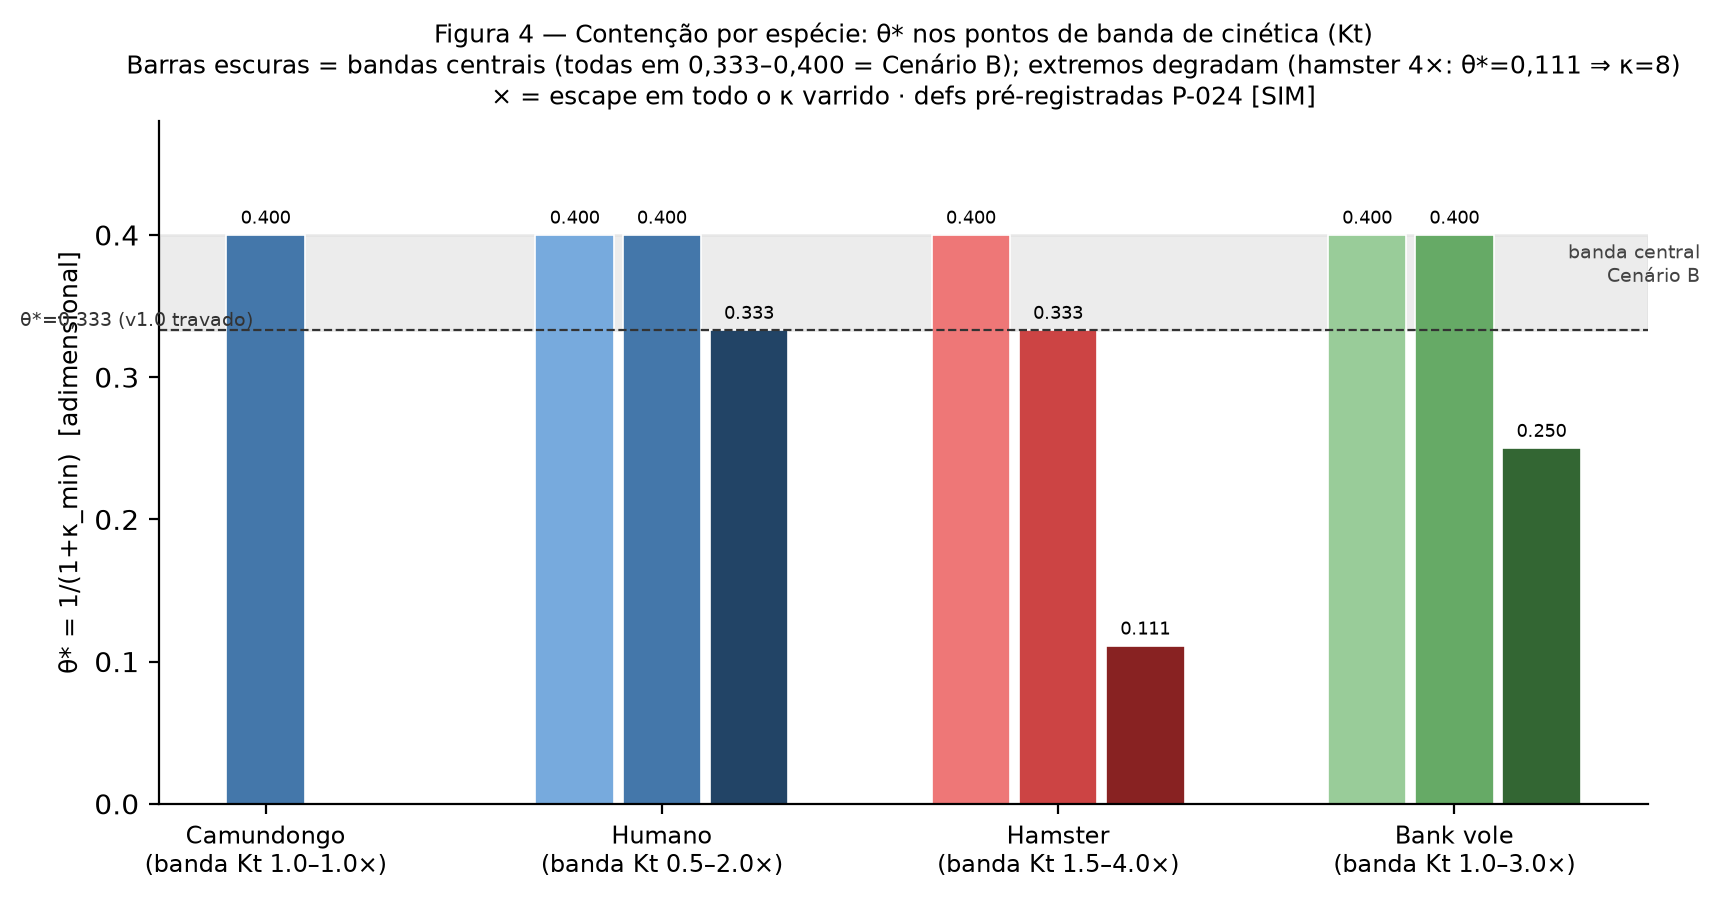
\includegraphics[width=0.9\textwidth,keepaspectratio]{../../paper/latex/figs/fig4_theta_species.png}}
\caption{Figura 4 --- θ* por espécie nas bandas de cinética}
\end{figure}

\emph{Figura 4 (auditável:
\texttt{experiments/xspecies/make\_fig4\_thetaspecies.py} lê somente os
JSONs p024; regenerável no CI). Proveniência integral: N-fatos
N055--N059; canon F-43/F-44; JSONs
\texttt{experiments/xspecies/p024\_\{mouse,human,hamster,vole\}.json}
(execução cloud 4/4, C0 exato por job).}

\begin{center}\rule{0.5\linewidth}{0.5pt}\end{center}

\chapter{APLICAÇÃO: O DESENHO TERAPÊUTICO
EMERGE}\label{aplicauxe7uxe3o-o-desenho-terapuxeautico-emerge}

\emph{Em linguagem clínica: com o fundamento validado (Cap. 3), o
desenho se completa --- onde depositar (anel 8--12 mm), com que malha, a
que intervalo (≤7 d), e agora: \textbf{quanta proteína por depósito},
como banda calculada com a incerteza declarada --- não como número
único. A dose permanece prognóstico {[}SIM{]} até o ensaio G0; o que
este capítulo entrega é o prognóstico quantitativo do braço
discriminador A6.}

Transporte: três regras falseáveis {[}SIM{]}

O solver de transporte (advecção--difusão--reação em meio poroso
heterogêneo; α=0,20 e λ=1,8 in-vivo; D\_eff=3,86×10⁻¹¹ m²/s;
auto-testado: conservação de massa 100,0\%, erro de Thiele 0,5\%) produz
as três regras de design:

\begin{enumerate}
\def\labelenumi{\arabic{enumi}.}
\tightlist
\item
  \textbf{Anel de contenção}: espaçamento inter-depósito \textbf{8--12
  mm} (raio de proteção r₁₀\%=2,303ℓ; ℓ=3,59 mm);
\item
  \textbf{Malha do veículo}: hidrogel com malha ξ≥5× o raio da proteína
  (HA 1--2\% p/p passa; \textgreater5\% sequestra);
\item
  \textbf{Redose}: intervalo \textbf{≤7 dias} para mRNA/LNP (trough
  ≥30--56\%; meia-vida de PrP 4,8--6,4 d).
\end{enumerate}

O limiar travado e a dose legitimada pela banda

A contenção exige θ = (1+κ·c\_pico)⁻¹ ≤ \textbf{θ*=0,333} (predição
travada no release v1.0 de 26/08; comparada, nunca retreinada). A
validação multi-espécie (Cap. 3) legitimou a dose κ=2 do desenho
original \textbf{dentro da banda humana herdada} (κ\_min=2,0 em Kt=2) e
a estendeu além dela pela regra de titulação κ\_req↔Kt --- com a
ressalva de horizonte sempre citada (seção 5.4).

Restava o elo que a Parte 1 declarara ilustrativo: \textbf{quanto vale κ
em massa?} Este capítulo o fecha como \textbf{banda} --- com critérios
de aceitação pré-registrados antes de qualquer computação (protocolo
garantista: toda célula da cadeia com unidade+fonte; banda sempre ≥2
extremos; a largura da banda dominada pelo elo κ↔µM (assumido
ilustrativo) é resultado válido e esperado; saída de planejamento,
jamais prescrição).

A primeira dose calculada: banda de dose do braço A6
{[}SIM-planejamento{]}

\textbf{Cadeia dimensional (todas as células com unidade+fonte; JSON
canônico \texttt{experiments/m31/m31\_u1u2.json} \cite{e58}):} κ\_req
(regra de titulação) → concentração no pico do depósito c = κ\_req × Kd
→ quantidade por depósito n = c × V\_halo → massa = n × MW. A banda do
Kd aparente é \textbf{0,071--1,0 µM} \emph{(illustrative assumption;
closed by arm A6)}: o piso, 71 nM, é o Kd medido por SPR para oligômeros
de Aβ42 ligando PrP humano \cite{e57} --- \textbf{proxy declarado}, pois
o par V127↔PrP\^{}Sc não tem Kd medido; o teto, 1 µM, é a âncora
ilustrativa da Parte 1 seção 2.2 \emph{(não é estimativa de secreção
medida)}. O volume do halo é um cilindro r×h com r₁₀\%=4--6 mm e fração
ECS 0,15--0,25 (casca de 2 mm declarada Tipo-B). A massa molecular é
\textbf{22,83 kDa}, computada das nossas próprias sequências P04156
(resíduos 23--231, forma madura; V127 é variante de mesma massa, Δ=+14
Da). Fontes da cadeia: Kd-piso · V-halo · ECS · MW · titulação.

\textbf{Escada de dose por banda-Kt do hospedeiro} (banda sob âncora
ilustrativa; fechada pelo braço A6):**

{\def\LTcaptype{none} % do not increment counter
\begin{longtable}[]{@{}
  >{\raggedright\arraybackslash}p{(\linewidth - 8\tabcolsep) * \real{0.2000}}
  >{\raggedright\arraybackslash}p{(\linewidth - 8\tabcolsep) * \real{0.2000}}
  >{\raggedright\arraybackslash}p{(\linewidth - 8\tabcolsep) * \real{0.2000}}
  >{\raggedright\arraybackslash}p{(\linewidth - 8\tabcolsep) * \real{0.2000}}
  >{\raggedright\arraybackslash}p{(\linewidth - 8\tabcolsep) * \real{0.2000}}@{}}
\toprule\noalign{}
\begin{minipage}[b]{\linewidth}\raggedright
Banda-Kt
\end{minipage} & \begin{minipage}[b]{\linewidth}\raggedright
κ\_req
\end{minipage} & \begin{minipage}[b]{\linewidth}\raggedright
c no pico (µM)
\end{minipage} & \begin{minipage}[b]{\linewidth}\raggedright
µg V127ΔGPI/depósito
\end{minipage} & \begin{minipage}[b]{\linewidth}\raggedright
Redose
\end{minipage} \\
\midrule\noalign{}
\endhead
\bottomrule\noalign{}
\endlastfoot
Kt 1 & 1,5 & 0,11--1,5 & 0,0--1,9 & ≤7 d \\
\textbf{Kt 2 (humano central)} & \textbf{2} & \textbf{0,14--2,0} &
\textbf{0,0--2,6} & \textbf{≤7 d} \\
Kt 3 & 3 & 0,21--3,0 & 0,1--3,9 & ≤7 d \\
Kt 4 (pior caso declarado) & 8 & 0,57--8,0 & 0,2--10,3 & ≤7 d \\
\end{longtable}
}

No degrau humano, a dose de A6 é \textbf{0,0--2,6 µg de V127ΔGPI por
depósito} (redose ≤7 d; regra 3); a escada sobe monotonicamente com
κ\_req até o pior caso declarado κ=8 (que cobre Kt=4): 0,2--10,3
µg/depósito.

\textbf{A largura da banda é o achado.} A razão pior/otimista é
≈\textbf{53× em todos os degraus} --- constante porque κ\_req cancela na
razão: ela decompõe-se em \textbf{14× do proxy de Kd} (71 nM → 1 µM;
assumido ilustrativo) × \textbf{3,7× do volume do halo} (4--6 mm; ECS
0,15--0,25). Isto não é defeito do cálculo: é a \textbf{quantificação
honesta do que o ensaio G0-A6 fecha} --- o braço de proteína
recombinante a dose conhecida converte a âncora κ↔µM de ilustrativa em
medida, colapsando a banda em ponto. Até lá, a dose existe como banda, e
a banda é planejamento {[}SIM{]}: prognóstico calculado, \textbf{não
prescrição}.

\begin{figure}[htbp]
\centering
\pandocbounded{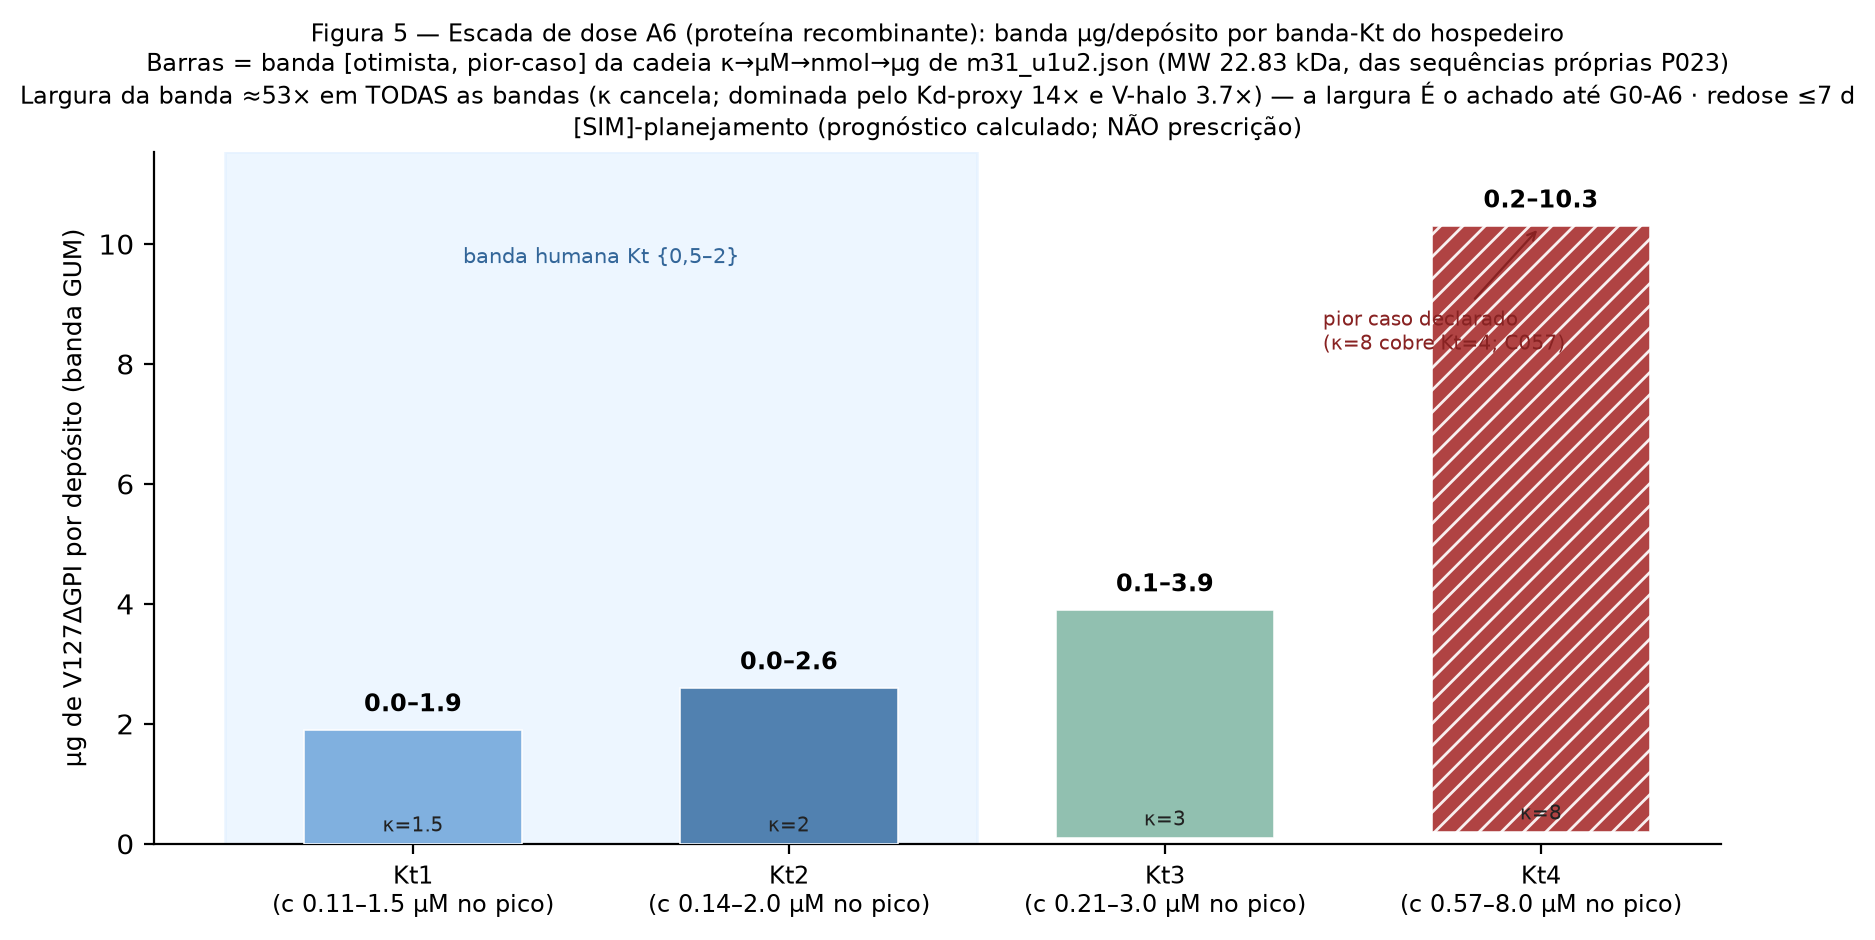
\includegraphics[width=0.9\textwidth,keepaspectratio]{../../paper/latex/figs/fig5_dose_ladder.png}}
\caption{Figura 5 --- Escada de dose A6: banda GUM µg/depósito por
banda-Kt}
\end{figure}

\emph{Figura 5 (auditável:
\texttt{experiments/m31/make\_fig5\_doseladder.py} lê somente
\texttt{m31\_u1u2.json}; regenerável no CI). Barras = banda {[}otimista,
pior-caso{]}; hachura = pior caso declarado κ=8 (C057); faixa azul =
banda humana Kt \{0,5--2\}; largura ≈53× constante (κ cancela) --- a
largura É o achado até G0-A6. Tier {[}SIM{]}-planejamento no título da
figura.}

\textbf{Por que A6 é o vetor-primário da dose:} por vetor, a unidade de
dose difere (A5 = células+secretor; A7 = µg de mRNA); apenas A6
(proteína recombinante) tem \textbf{dose conhecível de saída}. É o braço
discriminador: fecha o elo κ↔µM \emph{(illustrative assumption; closed
by arm A6)} e testa a forma funcional do capping (primeira potência vs
quadrática, travada na colheita {[}SIM{]} da Parte 1). A5 e A7 herdam a
cadeia como derivadas.

O ensaio que fecha a banda: G0-wet especificado

Oito braços pré-registrados (incluindo PPS como controle positivo
publicado e braço LNP-mRNA), com plano estatístico cego (Welch/Holm
α=0,05; 5 comparações; n=8→12; poder \textasciitilde80\% para Δ≥50\%),
cegamento do scorer, randomização estratificada por lote, kill-switches
por braço + critério de morte programática, contrato de dado
{[}ORGANOID{]} bancada→estimador (exclusões publicadas nunca editadas),
e o loop de re-parametrização que recalibra \textbf{exatamente o que o
dado informa}. Os dez itens de freeze F1--F10 com GATE-F de liberação
estão no Apêndice C; a especificação integral no registro.

Custo-cotação

A tabela suplementar S1 (custo por braço, cotações de mercado
arquivadas) está no Apêndice E --- o desenho é especificado ao ponto de
orçamento, sem executar compra.

\begin{center}\rule{0.5\linewidth}{0.5pt}\end{center}

\chapter{MÉTODOS: A ETRIZAÇÃO
FORMALIZADA}\label{muxe9todos-a-etrizauxe7uxe3o-formalizada}

Pipeline do método (P0--P6)

\textbf{Fluxo:} \textbf{P0} identificação (SLR auditada → base
E-registrada com linhagem) → \textbf{P1} parametrização (derivação com
proveniência por parâmetro) → \textbf{P2} execução (motores
determinísticos auto-testados → runs arquivados {[}SIM{]}) → \textbf{P3}
colheita (critérios pré-declarados → veredito sem meta móvel) →
\textbf{P4} prognóstico (predições travadas por release ANTES da medição
→ âncora anti-hindsight) → \textbf{P5} pesquisa derivada (novas
perguntas prosseguem imediatamente) → \textbf{P6} confronto opcional
(dado real análogo ⇒ antecipação bancada).

\emph{Tabela completa com entradas/saídas/garantias por passo: seção
7.1.}

O método nomeado: etrização computacional, passos P0--P6

\textbf{Inovação metodológica declarada:} avaliação computacional como
método antecipatório --- previsibilidade e antecipação de informação
para decisão de pesquisa (o que medir, onde, em que dose, antes de
gastar recurso). A \textbf{parametrização} (operação técnica do P1) é o
núcleo operacional; a \textbf{tese etrizada} é o produto. Declaração de
eixo retórico (obrigatória): tudo aqui \textbf{é simulação, e é dito que
é}; não se promete aplicar nem validar --- antes: \textbf{se dados reais
exibirem resultados análogos aos simulados, os passos seguintes já terão
sido dados} (antecipação bancada, não pendente).

{\def\LTcaptype{none} % do not increment counter
\begin{longtable}[]{@{}
  >{\raggedright\arraybackslash}p{(\linewidth - 10\tabcolsep) * \real{0.1667}}
  >{\raggedright\arraybackslash}p{(\linewidth - 10\tabcolsep) * \real{0.1667}}
  >{\raggedright\arraybackslash}p{(\linewidth - 10\tabcolsep) * \real{0.1667}}
  >{\raggedright\arraybackslash}p{(\linewidth - 10\tabcolsep) * \real{0.1667}}
  >{\raggedright\arraybackslash}p{(\linewidth - 10\tabcolsep) * \real{0.1667}}
  >{\raggedright\arraybackslash}p{(\linewidth - 10\tabcolsep) * \real{0.1667}}@{}}
\toprule\noalign{}
\begin{minipage}[b]{\linewidth}\raggedright
Passo
\end{minipage} & \begin{minipage}[b]{\linewidth}\raggedright
Nome
\end{minipage} & \begin{minipage}[b]{\linewidth}\raggedright
Entrada
\end{minipage} & \begin{minipage}[b]{\linewidth}\raggedright
Procedimento
\end{minipage} & \begin{minipage}[b]{\linewidth}\raggedright
Saída
\end{minipage} & \begin{minipage}[b]{\linewidth}\raggedright
Garantia
\end{minipage} \\
\midrule\noalign{}
\endhead
\bottomrule\noalign{}
\endlastfoot
P0 & identificação & pergunta focal & SLR auditada de dados publicados
validados & base E-registrada (58 fontes) & linhagem completa (seção
7.3) \\
P1 & parametrização & base E-registrada & derivação física/estatística
com proveniência por parâmetro & modelos parametrizados & cada número
amarra a fonte \\
P2 & execução & modelos & motores determinísticos, código aberto,
self-tests & runs arquivados {[}SIM{]} & reprodução entre ambientes \\
P3 & colheita & runs & critérios de aceitação pré-declarados &
resultados {[}SIM{]} + margens & veredito sem meta móvel \\
P4 & prognóstico & resultados & predições travadas por release antes de
qualquer medição & limiares/tabela-decisão & âncora anti-hindsight \\
P5 & pesquisa derivada & valores razoáveis & novas perguntas derivam
imediatamente & agenda derivada {[}SIM{]} & geração, não espera \\
P6 & confronto (opcional) & dados reais futuros, se análogos &
comparação à âncora travada (nunca retreino) & passos seguintes já
avançados & antecipação bancada \\
\end{longtable}
}

\textbf{Posição na família:} a etrização é irmã da meta-análise (agrega
o publicado), da modelagem física (deriva comportamento) e dos in-silico
trials (executa cenários) --- e distingue-se por \textbf{travar
prognósticos antes da medição e declarar a simulação como simulação em
cada saída} (tiers {[}SIM{]}/{[}ORGANOID{]}/{[}MOUSE{]}/{[}HUMAN{]}).

Formulação matemática com proveniência

\emph{Em linguagem clínica: as equações abaixo são o ``rastreio
farmacocinético'' da proteína no cérebro --- para onde difunde, quanto
dura, quão forte compete com o príon. Se você entende isso e as Figuras
4--5, a matemática é opcional: ela formaliza o que já foi dito em
palavras --- cada equação carrega a citação de onde veio cada
parâmetro.}

\textbf{Transporte (ADR) em meio poroso heterogêneo} (volumes finitos 2D
192², Euler explícito):

\[\frac{\partial(\alpha c)}{\partial t} = \nabla\!\cdot\!(D_{\mathrm{eff}}\,\nabla c) \;-\; \nabla\!\cdot\!(\mathbf{v}\,c) \;+\; S(\mathbf{x}) \;-\; k_{\mathrm{eff}}\,c\]

com α=0,20 e λ=1,8 medidos in-vivo; D\_eff=D₀/λ²=3,86×10⁻¹¹ m²/s
(D₀=1,25×10⁻¹⁰ m²/s, Stokes--Einstein, R\_h≈2,5 nm); k\_eff varrido
10⁻⁶--10⁻⁵ s⁻¹ ancorado à polimerização nucleada; fluxo intersticial por
Darcy; cistos espongiformes κ×50. Auto-testes: conservação de massa
100,0\%; erro de Thiele 0,5\% (ℓ=3,59 mm).

\textbf{Capping dominante-negativo e o limiar θ} (termo próprio):

\[\mathrm{freeS}(r) = \left(1 + \kappa\, c_{\mathrm{V127}}(r)\right)^{-2}, \qquad c_{\mathrm{V127}}(r) \propto e^{-r/\ell}, \qquad \theta \equiv \left(1 + \kappa\, c_{\mathrm{pico}}\right)^{-1} \in (0,1]\]

θ é a fração de atividade máxima de replicação no pico secretor;
contenção quando a frente assintótica cai \textless50\% do baseline
(T3). A forma quadrática reflete conversão de dois participantes; a
alternativa de primeira potência é falseável pela dose-resposta do braço
A6.

\textbf{Relógio humanizado} (âncoras de organoide): duplicação ≈12,1 d;
1 unidade-simulação = 144 d.

\textbf{Estimador θ\_obs}: features (raio R, log-razão de biomassa); κ̂
vizinho-mais-próximo na grade κ∈\{1,5--8\}; θ̂=1/(1+κ̂); regime por braço
(mediana, n=8, IC bootstrap 90\%). Veredito pré-declarado: ADEQUADO na
fronteira de decisão (cobertura 3/3; bias −0,008 em κ=2); v1.1
interpolada testada e rejeitada.

Base de Validade (MANDATÓRIA)

\textbf{Declaração tríade:} (i) esta tese é \textbf{baseada em simulação
computacional e NÃO SUBSTITUI a validação de laboratório} --- o
laboratório é essencial; (ii) a continuidade provém dos prognósticos: se
o G0-wet equivaler ao simulado, a antecipação já estará bancada; (iii) o
rigor experimental é \textbf{convertido para o ambiente computacional}:
cada dado com linhagem completa
(quem→espécie→cruzamento→código→parâmetro→resultado).

{\def\LTcaptype{none} % do not increment counter
\begin{longtable}[]{@{}
  >{\raggedright\arraybackslash}p{(\linewidth - 12\tabcolsep) * \real{0.1429}}
  >{\raggedright\arraybackslash}p{(\linewidth - 12\tabcolsep) * \real{0.1429}}
  >{\raggedright\arraybackslash}p{(\linewidth - 12\tabcolsep) * \real{0.1429}}
  >{\raggedright\arraybackslash}p{(\linewidth - 12\tabcolsep) * \real{0.1429}}
  >{\raggedright\arraybackslash}p{(\linewidth - 12\tabcolsep) * \real{0.1429}}
  >{\raggedright\arraybackslash}p{(\linewidth - 12\tabcolsep) * \real{0.1429}}
  >{\raggedright\arraybackslash}p{(\linewidth - 12\tabcolsep) * \real{0.1429}}@{}}
\toprule\noalign{}
\begin{minipage}[b]{\linewidth}\raggedright
Dado
\end{minipage} & \begin{minipage}[b]{\linewidth}\raggedright
Primário
\end{minipage} & \begin{minipage}[b]{\linewidth}\raggedright
Espécie/sistema
\end{minipage} & \begin{minipage}[b]{\linewidth}\raggedright
Cruzamento independente
\end{minipage} & \begin{minipage}[b]{\linewidth}\raggedright
Código
\end{minipage} & \begin{minipage}[b]{\linewidth}\raggedright
Parametrização humana
\end{minipage} & \begin{minipage}[b]{\linewidth}\raggedright
Resultado {[}SIM{]}
\end{minipage} \\
\midrule\noalign{}
\endhead
\bottomrule\noalign{}
\endlastfoot
Cinética de replicação & Fornara/Igel 2024 (aberto) {[}E009{]} &
camundongo & Masel 1999 {[}E011{]} & kernel portado & relógio às âncoras
humanas & θ*=0,333 {[}C038{]} \\
Relógio/amplitude humanos & Groveman 2019 {[}E007{]} & organoide sCJD &
Groveman 2021 {[}E008{]}; subtipos 2023 & regressão 12,1 d; 144 d/unid &
direto & predição θ\textless0,33 {[}C040{]} \\
Transporte intersticial & Thorne \& Nicholson 2006 {[}E010{]} & humano
in-vivo & Stokes--Einstein & solver ADR auto-testado & direto & regras
1--3 {[}C033-C035{]} \\
Agente V127 anchorless & Asante 2015 {[}E001{]} · Gatdula 2026
{[}E003{]} · Zerbes 2026 {[}E004{]} & população→camundongo→cultura→AAV &
quatro níveis independentes & termo freeS & dose↔κ em banda (seção 6.3)
& contenção κ=2 {[}C038{]} \\
Âncora κ↔µM (banda) & Chen 2010 SPR {[}E057{]} + âncora ilustrativa P1
seção 4.2 & humano (Aβ42-PrP; PROXY declarado) & --- & cadeia
dimensional M3.1 {[}E058{]} & direto & banda A6 0,0--2,6 µg
{[}C058-C060{]} \\
Prior de falhas clínicas & Geschwind 2013 · Haïk 2014 · Newman 2014 ·
Otto 2004 · Mead 2022 · Cheng 2015 {[}E034-E038, E022{]} & humano &
registry-bound & Beta--Binomial WS-8 & direto & P=5\%/30--45\% \\
Sensibilidade estrutural & (este programa) & in-silico & motor
reproduzido 2× (hash+valor) & sweeps S1-S3 + estimador & --- & predição
discriminadora {[}C051{]} \\
\end{longtable}
}

\textbf{Por que isto é ciência com referências sólidas:} toda célula
amarra fonte peer-reviewed ou run arquivado com hash; nenhum número vive
fora do registro (\textbf{60 claims · 58 fontes · 65 N-fatos · 4
validadores em zero · AST 9/9}); a cadeia é verificável de ponta a
ponta, como um ``métodos'' experimental exige.

A tese em forma experimental (mapeamento análogo)

{\def\LTcaptype{none} % do not increment counter
\begin{longtable}[]{@{}
  >{\raggedright\arraybackslash}p{(\linewidth - 2\tabcolsep) * \real{0.5000}}
  >{\raggedright\arraybackslash}p{(\linewidth - 2\tabcolsep) * \real{0.5000}}@{}}
\toprule\noalign{}
\begin{minipage}[b]{\linewidth}\raggedright
Tese experimental (com pessoas)
\end{minipage} & \begin{minipage}[b]{\linewidth}\raggedright
Esta tese (etrização)
\end{minipage} \\
\midrule\noalign{}
\endhead
\bottomrule\noalign{}
\endlastfoot
Participantes recrutados & Fontes publicadas (58 E-registradas) \\
Critérios de inclusão/exclusão & SLR auditada (query bank
pré-registrada) \\
Consentimento/aprovação ética & Proveniência aberta (identifier
confirmado) \\
Instrumentos calibrados & Código auto-testado (massa 100\%; ℓ 0,5\%) \\
Protocolo executado & P1 parametrização + P2 execução determinística \\
Dados coletados & Runs arquivados {[}SIM{]} (reprodução 2 ambientes) \\
Prontuário & Registro da tese (60 claims · 65 N-fatos · pendências
estruturadas) \\
Análise pré-especificada & P3 colheita + estimador θ\_obs calibrado \\
Implicações relatadas & P4 prognóstico + P5 derivada + P6 antecipação \\
Auditoria/supervisão & Guardião (4 dimensões de revisão hostil) \\
\end{longtable}
}

\emph{Um examinador que sabe ler tese experimental sabe ler esta: basta
trocar ``pessoa''→``fonte'', ``instrumento''→``código'',
``coleta''→``run'' --- a forma documental é idêntica; a base é simulação
computacional.} (Hipótese H1, testável: a auditoria trocando apenas os
termos do mapeamento não perde a tese.)

\begin{center}\rule{0.5\linewidth}{0.5pt}\end{center}

\chapter{RESULTADOS COMO VALIDAÇÃO (+ componentes
M1--M5)}\label{resultados-como-validauxe7uxe3o-componentes-m1m5}

\emph{Cada seção de resultados valida uma promessa declarada da tese;
nenhum resultado é métrica órfã.}

{\def\LTcaptype{none} % do not increment counter
\begin{longtable}[]{@{}
  >{\raggedright\arraybackslash}p{(\linewidth - 4\tabcolsep) * \real{0.3333}}
  >{\raggedright\arraybackslash}p{(\linewidth - 4\tabcolsep) * \real{0.3333}}
  >{\raggedright\arraybackslash}p{(\linewidth - 4\tabcolsep) * \real{0.3333}}@{}}
\toprule\noalign{}
\begin{minipage}[b]{\linewidth}\raggedright
Promessa (contribuição)
\end{minipage} & \begin{minipage}[b]{\linewidth}\raggedright
Resultado que a valida
\end{minipage} & \begin{minipage}[b]{\linewidth}\raggedright
Registro
\end{minipage} \\
\midrule\noalign{}
\endhead
\bottomrule\noalign{}
\endlastfoot
Existe um limiar de contenção quantitativo & θ*=0,333 travado v1.0; R
2,83→0,82 mm em κ=2; monotônico à quase-extinção & \\
O desenho é quantitativo (dose-e-posicionamento) & regras 1--3 (anel
8--12 mm; malha ≥5×r\_p; redose ≤7 d) & \\
O método é robusto a parâmetros não-medidos & sweeps S1/S2 (C50
insensível 10×); S3 (só Kt move contenção/relógio, Kr/Kc ≤3\%) & ·
F-43 \\
O limiar transfere entre espécies & Cenário B: θ* 0,333--0,400 centrais
(razão 1,20); refutação do hamster reportada como está & \\
A dose generaliza por cinética & regra de titulação κ\_req↔Kt
(1→1,5·2→2·3→3·4→8) & \\
A dose é calculável em massa com incerteza honesta & banda A6 0,0--2,6
µg/depósito (humano); largura ≈53× decomposta (14× Kd-proxy × 3,7×
V-halo) & \\
O instrumento de confronto funciona & θ\_obs ADEQUADO na fronteira (bias
−0,008); v1.1 rejeitada & \\
A decisão é possível sem dado novo & tabela-decisão derivada
(κ↔θ\_obs↔R↔biomassa); biomassa = coordenada informativa & \\
\end{longtable}
}

Os resultados da tese são os resultados da simulação já realizada

\textbf{Figuras da tese} (geradas dos JSONs arquivados por scripts
commitados --- regra: valor só de dado):

\begin{itemize}
\tightlist
\item
  \textbf{Figura 1} --- Resposta de contenção: raio assintótico R vs κ
  com os tiers T2/T3 anotados
  (\texttt{paper/latex/figs/fig2\_theta\_response.png}).
\item
  \textbf{Figura 2} --- Consistência emergente de subtipos
  MV2\textgreater MV1 (painéis frente contida + âncoras de semente 126×,
  entrada sem ajuste) (\texttt{paper/latex/figs/fig3\_subtypes.png}).
\item
  \textbf{Figura 3 (tabela-decisão)} --- derivada sem nova simulação: κ
  ↔ θ\_obs ↔ R ↔ razão de biomassa ↔ margem vs baseline
  (\texttt{experiments/part2\_results/part2\_derived\_summary.json};
  seção 6.1).
\item
  \textbf{Figura 4} --- θ* por espécie nos pontos de banda de cinética
  (Kt): banda central Cenário B sombreada (0,333--0,400); extremos
  degradam (hamster 4× ⇒ κ=8; × = escape) --- gerada dos JSONs p024\_*
  por script commitado
  (\texttt{paper/latex/figs/fig4\_theta\_species.png};
  \texttt{experiments/xspecies/make\_fig4\_thetaspecies.py}).
\end{itemize}

Em vez de laboratório ou teste humano, \textbf{o que valida e compõe a
tese neste estágio é o conjunto computacional executado} --- completo,
arquivado e reproduzido: (i) limiar de contenção θ*=0,333 com relógio
humanizado; (ii) três regras de design falseáveis; (iii) colheita de
sensibilidade com predição discriminadora (C₅₀ 10× insensível; forma
funcional falseável por dose-resposta); (iv) quadro probabilístico de
duas lentes com prior registry-bound; (v) estimador θ\_obs calibrado no
regime declarado; (vi) reprodução independente em dois ambientes (hash +
valor-a-valor); e (vii) a \textbf{tabela-decisão derivada}
(κ↔θ\_obs↔frente↔biomassa↔margem) extraída sem nova simulação --- que
mostra a margem de raio saturando cedo (70,2\% já em κ=1,5) e confirma a
\textbf{razão de biomassa como coordenada informativa} (48→1,25), com
θ*=0,333 como variável-de-decisão pré-registrada. De cada valor razoável
aqui, \textbf{pesquisa derivada já pode prosseguir} --- portas abertas.

M1 --- Estimador θ\_obs: o dado parametrizado como instrumento

O objetivo operacional: converter gradiente proximal/distal medido em
θ\_obs comparável ao limiar travado θ*=0,333 \textbf{sem circularidade}
(grade e função-objetivo congeladas antes do dado; Parte 1 seção 2.7). A
validação do próprio instrumento é computacional --- simulation-based
calibration sobre a grade κ∈\{1,5--8\} do motor v4 exato:

\begin{itemize}
\tightlist
\item
  \textbf{Calibração unitária} (1000 boots; ruído organoide publicado CV
  30/40\%): veredito \textbf{ADEQUADO} por critérios pré-declarados
  (cobertura do θ verdadeiro 3/3; bias ≤ 0,032) --- com nota honesta:
  resolução por-órganoide é baixa; a precisão vem do \textbf{regime
  declarado} (mediana por braço, n=8).
\item
  \textbf{Regime pooled n=8}: PASS integral \textbf{na fronteira de
  decisão} (κ=2: bias −0,008; recuperação modal 69\%; cobertura ✓) --- a
  região exata onde a predição travada decide (θ\textless0,33); em κ
  alto o bias é \textbf{conservador} (+0,060: superestima θ, subestima
  contenção --- erro no lado seguro).
\item
  \textbf{v1.1-IDW (interpolação) testada e rejeitada}: piorou a
  fronteira (bias −0,037, direção anti-conservadora) e quebrou cobertura
  em κ=8 --- registrado como evidência de que a disciplina
  anti-hindsight está viva: o upgrade que falha é descartado, não
  embranquecido.
\item
  Achado de design que o método produziu: a razão de biomassa carrega a
  informação que o raio perde por saturação (R 0,843→0,760 mm contra
  razão 48→1,25 na grade) --- o estimador opera no par de features por
  necessidade.
\end{itemize}

M2 --- Freeze de execução: o que trava antes do primeiro organoide

Dez itens F1--F10, com GATE-F de liberação: estimador (F1, fechado ---
Cap. 5), plano estatístico (Welch/Holm α=0,05, 5 comparações; n=8→12;
poder \textasciitilde80\% para Δ≥50\%), cegamento do scorer,
randomização/estratificação por lote (DP MV2 ≈77\% da média publicada),
controle positivo A8-PPS como critério de validade do ensaio,
kill-switches por braço + \textbf{critério de morte programática},
esquema de dado {[}ORGANOID{]} (contrato bancada→estimador; exclusões
publicadas nunca editadas), loop M3, timelines (readouts 90--120 d;
regime estacionário desde \textasciitilde4 d) e M4 (parceiro por
método). Regra: pós-GATE-F, qualquer mudança é emenda auditada com
re-análise com-e-sem.

M3 --- Loop de re-parametrização (o coração anti-hindsight)

O dado medido recalibra \textbf{exatamente o que informa}: o braço A6
(dose conhecida) fecha κ↔µM --- âncora ilustrativa da Parte 1 seção 2.2
tornado absoluto pelo dado --- convertendo o cálculo de contenção de
relativo a absoluto --- e executa o teste discriminador da forma
funcional (primeira potência vs quadrática; travado na colheita
{[}SIM{]} da Parte 1); θ* \textbf{compara-se, nunca se retreina}; taxas
murinas relativas e parâmetros de transporte humano só mudam por dado do
seu próprio escopo. Toda comparação cita a âncora do release onde a
predição foi travada (v1.0 / v3.0); toda recalibração gera pre-dição
nova \textbf{antes} do próximo dado --- o loop nunca ``explica depois''
sem ter previsto antes.

M4 --- Método de seleção de parceiro: assertividade por método
(SLR-análogo)

\textbf{A tese documenta o COMO; não seleciona o QUEM}. O protocolo
(v2.1) é o análogo de revisão sistemática aplicado à decisão ``onde
medir'':

\begin{enumerate}
\def\labelenumi{\arabic{enumi}.}
\tightlist
\item
  \textbf{Query bank Q1--Q5} --- strings exatas por plataforma (PubMed
  \texttt{{[}tiab{]}}, ClinicalTrials.gov, cinza-conferências, rede BR),
  registradas antes da execução, ancoradas em commit (PROSPERO-análogo);
\item
  \textbf{Inclusão I1--I5 / exclusão X1--X4 binárias} --- plataforma
  organoide-príon publicada · BSL-príon certificada · capacidade ≥64
  organoides com controle de lote · aceitação de
  pré-registro/kill-switch · formalização ≤6 meses; vetos: sem
  biossegurança, sem cegamento, IP exclusiva, indisponibilidade
  \textgreater12m;
\item
  \textbf{Pesos congelados A--H} (25/15/15/10/10/10/10/5 --- plataforma,
  track príon, capacidade, braço A5, braço A7, co-localização BR/E200K,
  open-science, prontidão), âncoras 0--5, ``?'' não pontua por regra;
\item
  \textbf{Fluxo PRISMA-regenerável}
  (identificados→dedup→triagem→pontuação→contato sequencial por score;
  desempate = plataforma) com log datado e público;
\item
  \textbf{Aplicação-piloto} (log v0.2): demonstra executabilidade --- 9
  registros → 8 grupos → 2 elegíveis + 1 condicional + 3 watchlist + 2
  técnicos; o método corrigiu o prior (peso do eixo D em Calgary à luz
  do JCI 2026); o piloto \textbf{não decide} --- as ordens que emite são
  saídas do método para o executor futuro.
\end{enumerate}

Replicabilidade posterior: qualquer pesquisador re-executa as strings,
re-tria, re-pontua; divergências \textgreater10 pts viram auditoria, não
erro. Viés declarado: single-rater v1 (co-rating pré-declarado como
pendência).

M5 --- Infraestrutura de continuidade (guardião + runbook)

O guardião opera com \textbf{perfis de superfície}
(\texttt{-\/-profile\ part1\textbar{}part2}): a Parte 2 tem contrato
próprio de gate (mesmo registro de pendências estruturado, baterias e
binding de números citados; sem herdar os padrões literais da Parte 1),
e a \textbf{Base de Validade (seção 7.3) é check BLOCKED permanente}
neste perfil. Toda superfície de manuscrito é gated por revisão hostil
recursiva (R0 drift estrutural · R1 checklist+baterias · R2 recursão de
emendas · R3 interrogação epistêmica + registro 〔a preencher pela
autora: id〕); o decálogo vivo (tiers de dado · locked-stays-locked ·
ilustrativo≠evidência · paridade · anti-hindsight ·
fim-de-sessão=/RECAP) está no guardian.md com comandos copy-paste --- a
continuidade não depende de memória de quem continua, e sim de método
documentado --- índice-mestre no KNOWLEDGE\_CANON.md.

\begin{center}\rule{0.5\linewidth}{0.5pt}\end{center}

\chapter{ACHADOS, IMPACTOS E ÁREAS CORRELATAS; PRÓXIMAS
ABORDAGENS}\label{achados-impactos-e-uxe1reas-correlatas-pruxf3ximas-abordagens}

Este capítulo responde à pergunta ``e daí?'': consolida os achados,
mapeia os impactos em camadas, identifica as áreas correlatas onde o
mesmo método é aplicável, e declara --- mandatoriamente --- o que vem a
seguir.

Achados e impactos

\textbf{Achados {[}SIM{]} consolidados:} o limiar adimensional θ*=0,333
(contenção acima dele, monotônica à quase-extinção); três regras de
design quantitativas (anel 8--12 mm; malha ≥5×r\_p; redose ≤7 d); a
predição discriminadora (a dose-resposta do braço A6 distingue a unidade
inibitória molecular); o estimador θ\_obs calibrado na fronteira de
decisão; a tabela-decisão derivada (biomassa como coordenada
informativa; raio saturado); e a validação multi-espécie (Cenário B +
regra de titulação κ↔Kt + dependência de horizonte).

\textbf{Impactos por camada:} (i) \emph{direto (DCJ)} --- primeiro
dimensionamento quantitativo de entrega para uma doença 100\% fatal, com
população-âncora E200K-Brasil e rota compassiva acelular desenhada; (ii)
\emph{plataforma (prion-like: AD/PD, \textgreater50M)} --- o cálculo
(campo secretor → limiar → posicionamento → calendário) é agnóstico de
proteína, transferível como framework de design --- explicitamente
gerador-de-hipótese; (iii) \emph{meta-científico} --- a etrização
demonstrada de ponta a ponta com auditoria de máquina: como continuar
pesquisa com rigor antes e independente da confirmação (iii-bis)
\emph{epistemológico} --- a etrização nomeia e legitima uma categoria de
conhecimento que a saúde produz mas não reconhecia: o prognóstico
quantitativo simulado-com-dados-reais como forma autônoma e disciplinada
de saber (não promessa, não hipótese --- \textbf{conhecimento
potencial-verificável com data de validade declarada}).

\subsection{5.1-bis. O achado único inovador: cura +
restauração}\label{bis.-o-achado-uxfanico-inovador-cura-restaurauxe7uxe3o}

\textbf{O achado único inovador --- dupla potencialidade terapêutica:}
1. \textbf{Cura da doença priônica}: contenção do espalhamento de
PrP\^{}Sc pelo mecanismo dominante-negativo V127 --- impedir a
propagação é interromper a cascata neurodegenerativa; 2.
\textbf{Restauração neurológica}: evidência da Parte 1 demonstra que
NPCs integram e \textbf{restauram parâmetros eletrofisiológicos} em
organoides CJD mesmo com príon ativo --- o componente celular não apenas
contém, mas \textbf{resgata função} na penumbra. A plataforma V127 é a
única abordagem antipriônica com este duplo potencial (conter +
restaurar).

\textbf{Ressalva mandatória}: estes achados \textbf{não podem ser
aplicados em humanos} apesar do potencial demonstrado --- faz-se
necessário, para uso humano, o teste e a validação com dados
experimentais da Parte 1 (pré-tese) executados em laboratório. A tese
entrega o prognóstico; a aplicação exige o G0-wet.

Áreas correlatas com a mesma usabilidade

O método da etrização aplica-se onde houver (a) base de dados publicados
e validados, (b) motor determinístico auditável e (c) decisão de
pesquisa sob incerteza: farmacologia de doenças raras (priorização de
dose/rota antes do primeiro animal); oncologia --- triagem de
combinações (ordenação de candidatos antes do ensaio); doenças
neurodegenerativas prion-like (o caso direto); toxicologia/regulação
(in-silico first, na linha dos frameworks regulatórios emergentes); e
qualquer programa que precise decidir \emph{o que medir, onde e em que
dose} antes de gastar recurso --- a função-objetivo da própria
etrização.

\subsection{5.2-bis. Replicabilidade demonstrada: como aplicar a
AD/PD}\label{bis.-replicabilidade-demonstrada-como-aplicar-a-adpd}

\textbf{Exemplo concreto de replicação para Alzheimer/Parkinson:} 1.
\textbf{P0-identificação}: SLR de dados publicados de propagação de
Aβ/α-sinucleína (Braak staging; ensaios de seeding RT-QuIC); 2.
\textbf{P1-parametrização}: modelo de difusão de agregados ao longo de
vias neurais (parâmetros de transporte análogos ao WS-7); 3.
\textbf{P2-execução}: simulação de intervenção (anticorpo anti-agregante
com campo secretor análogo ao V127ΔGPI); 4. \textbf{P4-prognóstico}:
limiar de contenção θ* para cada proteína --- travado antes de qualquer
dado; 5. \textbf{P5-derivada}: agenda de pesquisa sobre posicionamento
de infusão e dose --- gerada da simulação.

\textbf{Limitação declarada}: para Aβ/α-synucleína, NÃO existe variante
protetora natural selecionada pela evolução (como o V127 do kuru). O
agente terapêutico teria de ser engenheirado (anticorpo, variante
travada, degradação direcionada) --- uma incerteza adicional de
existência, não apenas de engenharia. O cálculo (P0-P5) transfere; o
agente, não.

Próximas abordagens (declaração mandatória conforme metodologia)

\textbf{Este trabalho foi realizado com base simulada.} Faz-se
\textbf{necessário o laboratório experimental e testes humanos para
validação} --- a simulação não substitui nem substituirá essa etapa
(seção 7.3). Contudo, \textbf{assim que dados humanos forem encontrados
--- independentemente dos valores que exibam --- eles podem ser
parametrizados contra os valores aqui obtidos} (loop de
re-parametrização, Cap. metodologia), o que \textbf{já representa um
passo à frente na pesquisa}: dado análogo confirma a antecipação (passos
seguintes já avançados, P6); dado divergente recalibra exatamente o que
informa, com a predição anterior preservada como âncora --- em ambos os
casos, conhecimento novo bancado.

\textbf{O que deve ser mandatoriamente realizado, conforme a
metodologia, para garantir resultados aplicáveis à sociedade:} (1)
execução do degrau {[}ORGANOID{]} pelo protocolo congelado (F1--F10;
GATE-F com assinatura de PI; estimador θ\_obs com scorer cego; plano
estatístico Welch/Holm; kill-switches por braço e programa); (2) degrau
{[}MOUSE{]} sob as regras de pivot pré-declaradas; (3) degrau
{[}HUMAN{]} exclusivamente pela via compassiva E200K com DSMB, endpoints
de contenção/desaceleração, comunicação responsável às famílias e
equidade de acesso à população-âncora; (4) em todos os degraus:
pré-registro antes do dado, publicação do resultado negativo quando
ocorrer, e rótulo de tier em toda saída. Nenhum atalho fora desta
sequência produz resultado aplicável --- é o que a metodologia exige e o
guardião atesta.

\emph{(adendo filosófico REALIZADO: a reflexão etrização/átomo da autora
--- registrada no corpus externo e integrada via Nota à Leitura, seção
7.1 nome-do-método, Cap. 9.3 declaração mandatória e Cap. 13 síntese ---
É o adendo; commit 83bbf51)}

\begin{center}\rule{0.5\linewidth}{0.5pt}\end{center}

\chapter{DISCUSSÃO}\label{discussuxe3o}

Este capítulo pesa os resultados: o que significam, o que não
significam, e como se posicionam entre a promessa e o limite.

Promessas e limites desta Parte 2

Promete: a etrização como método completo, replicável e em parte já
demonstrado (M1 executado; M4 piloto) --- continuar pesquisa por
simulação hoje, como a física, sem parar à espera de cada confirmação. E
declara: os resultados daqui \textbf{são de simulação e assim permanecem
rotulados}; a aplicação/validação em ambiente real não é prometida nesta
Parte --- se dados reais futuros forem análogos aos simulados,
\textbf{os passos seguintes já estão avançados} (P6). \textbf{Não
promete}: seleção de parceiro (execução externa), dado {[}ORGANOID{]}+
(não existe ainda --- e é rotulado como tal), nem qualquer claim clínica
(escada de tiers: nenhum degrau empresta a autoridade do seguinte).
Limites declarados: pesos e scores são julgamento estruturado
single-rater; a calibração do estimador é na grade atual (refinamento
futuro = grade mais fina, pré-declarado); PubMed-direto e identificação
R8 pendem como conformidade do piloto.

Discussão: o que os resultados significam e o que não significam

Os resultados {[}SIM{]} significam: (i) existe um limiar adimensional
(θ*=0,333) acima do qual o modelo contém a frente --- quantidade
comparável entre subtipos e, agora sondada computacionalmente entre
espécies (Cenário B: aproximadamente conservada nas bandas centrais, com
regra de titulação e declaração obrigatória de horizonte); (ii) o design
é quantitativo (anel 8--12 mm; malha ≥5×; redose ≤7 d) --- nenhum
candidato anterior o teve; (iii) o método é falseável em três frentes
pré-registradas (θ medido; C50 invariância; dose-resposta do A6
discriminando a forma funcional). Não significam: contenção em tecido
humano medido (isso é {[}ORGANOID{]}+, inexistente); eficácia clínica;
nem substituição do laboratório (seção 7.3). A contribuição de maior
alcance é a demonstração de que a própria continuidade da pesquisa pode
ser metodologicamente rigorosa sem parar à espera de confirmação --- a
etrização executada de ponta a ponta com revisão hostil de máquina e
validação expressa da autora.

\begin{center}\rule{0.5\linewidth}{0.5pt}\end{center}

\chapter{CAMADA CLÍNICA --- pré-abordagem dos temas antes da penetração
técnica}\label{camada-cluxednica-pruxe9-abordagem-dos-temas-antes-da-penetrauxe7uxe3o-tuxe9cnica}

\begin{quote}
⚠️ \textbf{PROGNÓSTICO {[}SIM{]} --- NÃO É CONSELHO MÉDICO.}
Documentação de desenho de pesquisa sob simulação parametrizada; nenhum
uso humano sem os gates {[}ORGANOID{]}→{[}MOUSE{]}→regulatório; nada
aqui orienta conduta, dose ou seleção de paciente. Verificação: autora
responsável + guardião de máquina (gates 0-BLOCKED).
\end{quote}

\textbf{Por que abrir estas páginas: doenças priônicas são 100\% fatais
e não têm hoje nenhuma terapia modificadora aprovada --- e este trabalho
traz o primeiro cálculo quantitativo de dose-e-entrega de um candidato,
com predições travadas antes de qualquer medição.}

\textbf{O que esta tese é, em cinco perguntas que qualquer médico
faria:}

\begin{enumerate}
\def\labelenumi{\arabic{enumi}.}
\tightlist
\item
  \textbf{Que doença?} Doenças priônicas (DCJ esporádica/genética):
  rapidamente progressivas, 100\% fatais, sem terapia modificadora
  aprovada --- seis candidatos já faliram em clínica.
\item
  \textbf{Que ideia?} Usar a variante PrP-G127V --- selecionada pela
  evolução (kuru) por proteger portadores --- como agente
  \textbf{dominante-negativo}: uma proteína que compete com o príon e
  trava sua replicação sem silenciar o PrP nativo (ao contrário dos ASOs
  em ensaio clínico).
\item
  \textbf{Que evidência?} Nenhuma medição nova em pacientes: a tese
  opera por \textbf{simulação parametrizada com dados reais publicados}
  (``etrização'') --- cada número vem de fonte rastreável; predições
  ficam travadas ANTES de qualquer medição futura (anti-hindsight).
\item
  \textbf{Que resultado prático?} Três regras de dosagem/posicionamento
  quantitativas (anel de depósitos 8--12 mm; redose ≤7 dias; limiar
  θ*≈⅓) + a sondagem multi-espécie: o limiar é \textbf{aproximadamente
  conservado} entre espécies (Cenário B), mas a dose exigida sobe com a
  velocidade da doença --- regra de titulação --- e, agora, \textbf{a
  primeira dose calculada do braço A6: banda de 0,0--2,6 µg de proteína
  por depósito no degrau humano (pior caso 0,2--10,3), com a largura da
  banda explicitando exatamente o que o ensaio organoide fecha}.
\item
  \textbf{Que promessa NÃO faz?} Não promete cura, aplicação humana, nem
  substitui laboratório: o prognóstico é entregue como conhecimento
  falseável; o uso humano exige o gate organoide (G0-wet) e além.
\end{enumerate}

\textbf{Como ler os símbolos sem perder o fio:} θ* = \emph{``quanto da
conversão sobrevive à dose no pior dia do anel''} (⅓ ≈ contém; ⅑ ≈ quase
extingue); κ = \emph{a dose}; Kt = \emph{a velocidade inerente da
doença}. Cada capítulo técnico abre com um parágrafo \textbf{``Em
linguagem clínica''} antes da formulação --- quem quiser pular a
matemática não perde o argumento.

\subsection{Resumo em 1 página --- rota de leitura de 10
minutos}\label{resumo-em-1-puxe1gina-rota-de-leitura-de-10-minutos}

\textbf{Rota:} (1) este capítulo (3 min) → (2) \textbf{Figura 4} --- a
dose-limiar por espécie (2 min) → (3) \textbf{Figura 5} --- a escada de
dose com a banda do braço A6 (2 min) → (4) Cap. 8 ``o que os resultados
significam e o que não significam'' (2 min) → (5) Cap. 13 conclusões por
objetivo (1 min).

\textbf{A mensagem inteira em três frases:} (i) a variante G127V, achada
pela evolução no kuru, pode travar a replicação do príon por competição
(dominante-negativo) sem silenciar a proteína nativa; (ii) a simulação
parametrizada com dados publicados entrega regras quantitativas de
dose-e-posicionamento (anel 8--12 mm · redose ≤7 d · limiar θ*≈⅓ · banda
A6 0,0--2,6 µg/depósito) com predições travadas ANTES de qualquer
medição --- o limiar aproximadamente conservado entre espécies (Cenário
B), dose titulada à velocidade da doença; (iii) nada disto é aplicável a
humanos antes do gate organoide (G0-wet) --- a não-promessa é parte do
método, não um enfeite.

\subsection{Acompanhamento previsto no desenho {[}SIM{]} (documentação
de desenho --- NÃO conduta
clínica)}\label{acompanhamento-previsto-no-desenho-sim-documentauxe7uxe3o-de-desenho-nuxe3o-conduta-cluxednica}

{\def\LTcaptype{none} % do not increment counter
\begin{longtable}[]{@{}
  >{\raggedright\arraybackslash}p{(\linewidth - 6\tabcolsep) * \real{0.2500}}
  >{\raggedright\arraybackslash}p{(\linewidth - 6\tabcolsep) * \real{0.2500}}
  >{\raggedright\arraybackslash}p{(\linewidth - 6\tabcolsep) * \real{0.2500}}
  >{\raggedright\arraybackslash}p{(\linewidth - 6\tabcolsep) * \real{0.2500}}@{}}
\toprule\noalign{}
\begin{minipage}[b]{\linewidth}\raggedright
O que o desenho prevê medir
\end{minipage} & \begin{minipage}[b]{\linewidth}\raggedright
Quando (previsto no desenho)
\end{minipage} & \begin{minipage}[b]{\linewidth}\raggedright
Instrumento declarado
\end{minipage} & \begin{minipage}[b]{\linewidth}\raggedright
Por quê
\end{minipage} \\
\midrule\noalign{}
\endhead
\bottomrule\noalign{}
\endlastfoot
θ\_obs (resposta à contenção in situ) & readouts 90--120 d (organoide) &
perfis radiais WB/IHC c/ leitura cega & critério de resposta
pré-registrado (θ\_obs\textless0,33) \\
Manutenção da cobertura secretora & redose ≤ 7 d (regra 3) & gradiente
proximal/distal & trough ≥30--56\% do pico {[}SIM{]} \\
Triagem pré-sintomática (população-âncora E200K) & --- & RT-QuIC + NfL &
precedentes tofersen/nusinersen (endpoint biomarcador) \\
\end{longtable}
}

\emph{Serviços de neurologia interessados em auditar ou viabilizar o
próximo gate encontram o pacote completo em
\texttt{paper/G0\_UNLOCK\_DOSSIER.md} +
\texttt{paper/lab\_outreach\_package.md} (nenhuma promessa de retorno
terapêutico).}

\begin{center}\rule{0.5\linewidth}{0.5pt}\end{center}

\chapter{LIMITAÇÕES COMO FRUTO (cada limite com o que o
fecha)}\label{limitauxe7uxf5es-como-fruto-cada-limite-com-o-que-o-fecha}

\emph{Reconhecer os limites com plano de pesquisa futura --- cada
limitação abaixo tem o gate/ensaio que a converte em conhecimento.}

\textbf{Classe de transferência (o dado é de outra espécie/sistema):} 1.
Cinética murina → humano: fechada em estrutura pelo Cenário B + relógio
humanizado; fechada em medida pelo G0-wet {[}ORGANOID{]}. 2. Âncora κ↔µM
é proxy \emph{(illustrative assumption; closed by arm A6)}: o Kd usado é
do par Aβ42-oligômero↔PrP, não do par V127↔PrP\^{}Sc. \textbf{A banda de
dose inteira (largura ≈53×) quantifica este limite} --- fechada pelo
braço A6 (dose conhecida). 3. Sem dado {[}ORGANOID{]}+ medido: G0-wet
especificado (F1--F10; GATE-F).

\textbf{Classe de horizonte (o número depende da janela de observação):}
4. θ* é dependente de horizonte (3 definições; Kt=2/κ=2 contém sob duas,
escapa sob a terceira): toda citação declara a def; a predição v1.0 usa
S3 --- fechada pela definição operacional no protocolo G0.

\textbf{Classe de estrutura-modelo:} 5. Escapes saturam no canto do grid
(2,83 mm): raio nesses braços é limite inferior --- grade maior
pré-declarada como refinamento. 6. Espécie reduz-se à banda Kt (por
construção): a disseminação das bandas É a pergunta multi-espécie;
refinamento por parâmetros por-espécie além de Kt é pesquisa derivada.
7. Forma funcional do capping (quadrática vs primeira potência) não
discriminada: falseável pela dose-resposta do A6.

\textbf{Classe de fontes monitoradas:} 8. Preprints/ensaios em andamento
(PRN100 extension; AAV-PrP) monitorados no registro; elevação a E-ID só
após abertura e verificação. 9. Ensaio retraído excluído por regra
(minociclina) --- a correção de citações recorrentes do campo é
subproduto auditável.

\textbf{Classe de execução:} 10. Single-rater nos pesos do protocolo de
parceiro (co-rating pré-declarado como pendência); PubMed-direto
pendente como conformidade do piloto.

\textbf{Classe de localização:} 11. População-âncora E200K-Brasil: a
rota compassiva depende de DSMB, equidade de acesso e comunicação
responsável --- especificada, não prometida.

\begin{center}\rule{0.5\linewidth}{0.5pt}\end{center}

\chapter{CONCLUSÕES POR OBJETIVO}\label{conclusuxf5es-por-objetivo}

\textbf{OE1 (nomear e formalizar a etrização) --- alcançado.} P0--P6 com
garantias por passo; nota à banca (Cap. 1) diferencia o termo de IST e
meta-análise.

\textbf{OE2 (Base de Validade) --- alcançado.} Tríade + linhagem
completa --- agora 7 linhas, incluindo a linha da âncora de conversão
κ-concentração \emph{(illustrative assumption; closed by arm A6)} em
banda.

\textbf{OE3 (resultados como achados {[}SIM{]}) --- alcançado.} Limiar;
regras 1--3; sensibilidade discriminadora; probabilístico; estimador na
fronteira; tabela-decisão; validação multi-espécie; \textbf{e a primeira
dose calculada com incerteza propagada} --- a banda A6 (0,0--2,6
µg/depósito no degrau humano; largura ≈53× = o que G0-A6 fecha) converte
a regra de dose da Parte 3 em prognóstico de massa.

\textbf{OE4 (continuidade documentada como método) --- alcançado.} Loop
anti-hindsight; seleção de parceiro SLR-análogo (método, não seleção);
freeze dormente.

\textbf{OE5 (revisão hostil + validação expressa) --- alcançado.} R0--R3
dois perfis 0 BLOCKED; AST 9/9; registro 60 claims · 58 fontes · 65
N-fatos.

\textbf{Hipóteses.} H1 corroborada no nível documental (mapeamento
análogo seção 7.4). H2 corroborada pelas predições travadas v1.0 e
refutações reportadas como estão (hamster; v1.1 do estimador). H3
corroborada pelo posicionamento estrutural (Cap. 1.2; Cap.
2-fundamentação da Parte 2).

\textbf{Síntese final.} Esta tese é uma \textbf{etrização} ---
realizada, rotulada e auditável. O método produziu-a a partir
exclusivamente de dados reais publicados e a entrega como prognóstico
falseável: limiar, regras, escada de dose em banda, e o ensaio que fecha
cada banda especificado. \textbf{Fecho epistemológico:} o que uma
pesquisadora pode legítimamente produzir quando a doença mata em meses,
o laboratório custa fortunas e os dados publicados estão disponíveis?
\textbf{Prognóstico quantitativo, falseável e disciplinado por
critérios} --- com nome (etrização), método (P0--P6), garantias (5
requisitos) e honestidade sobre o que é e o que não é. Como o átomo
tornou pesquisável o invisível, a etrização torna pesquisável o
ainda-não-medido.

\begin{center}\rule{0.5\linewidth}{0.5pt}\end{center}

\nocite{*}
\begin{thebibliography}{99}\setlength{\itemsep}{1pt}
\bibitem{e1} ASANTE, E.A. et al. A naturally occurring variant of the human prion protein completely prevents prion disease. 2015. doi:10.1038/nature14510.
\bibitem{e2} MEAD, S. et al. A novel protective prion protein variant that colocalizes with kuru exposure. 2009. doi:10.1056/NEJMoa0809716.
\bibitem{e3} GATDULA, J.R. et al. Leveraging the dominant-negative effect of the kuru-protective G127V prion protein variant as a novel therapeutic. 2026. PMID 41757113.
\bibitem{e4} ZERBES, T. et al. A self-complementary recombinant adeno-associated virus vector coding for an anchorless prion protein carrying. 2026.
\bibitem{e5} HOSSZU, L.P. et al. Structural effects of the highly protective V127 polymorphism on human prion protein. 2020. doi:10.1038/s42003-020-01126-6.
\bibitem{e6} ZHENG, Z. et al. Structural basis for the complete resistance of the human prion protein mutant G127V to prion disease. 2018. doi:10.1038/s41598-018-31394-6.
\bibitem{e7} GROVEMAN, B.R. et al. Sporadic Creutzfeldt-Jakob disease prion infection of human cerebral organoids. 2019. doi:10.1186/s40478-019-0742-2.
\bibitem{e8} GROVEMAN, B.R. et al. Human cerebral organoids as a therapeutic drug screening model for Creutzfeldt-Jakob disease. 2021. doi:10.1038/s41598-021-84689-6.
\bibitem{e9} FORNARA, B. et al. The dynamics of prion spreading is governed by the interplay between the non-linearities of tissue response and. 2024. PMID 39717079.
\bibitem{e10} THORNE, R.G. et al. In vivo diffusion analysis with quantum dots and dextrans predicts extracellular space and tortuosity in brain. 2006. doi:10.1073/pnas.0509425103.
\bibitem{e11} MASEL, J. et al. Quantifying the kinetic parameters of prion replication. 1999. doi:10.1016/S0301-4622(99)00004-3.
\bibitem{e12} WILLIAMS, K. et al. Neural cell engraftment therapy for sporadic Creutzfeldt-Jakob disease restores neuroelectrophysiological para. 2023. doi:10.1186/s13287-023-03591-2.
\bibitem{e13} RELANO-GINES, A. et al. Prion replication occurs in endogenous adult neural stem cells and alters their neuronal fate. 2013. doi:10.1371/journal.ppat.1003485.
\bibitem{e14} GINHOUX, F. et al. Fate mapping analysis reveals that hematopoietic cells of yolk-sac origin give rise to microglia. 2010. doi:10.1126/science.1194637.
\bibitem{e15} SORRELLS, S.F. et al. Human hippocampal neurogenesis drops sharply in children to undetectable levels in adults. 2018. doi:10.1038/s41586-018-0336-4.
\bibitem{e16} ABUD, E.M. et al. iPSC-derived human microglia-like cells to study neurological diseases. 2017. PMID 28426964.
\bibitem{e17} HAN, X. et al. Generation of hypoimmunogenic human pluripotent stem cells. 2019. doi:10.1073/pnas.1902566116.
\bibitem{e18} HU, X. et al. Hypoimmune induced pluripotent stem cells survive long-term in fully immunocompetent allogeneic rhesus macaque. 2024. doi:10.1038/s41587-023-01784-x.
\bibitem{e19} XUE, Y. et al. Lipid nanoparticles enhance mRNA delivery to the central nervous system upon intrathecal injection. 2025. PMID 40317512.
\bibitem{e20} LIANG, Y. et al. The survival of engrafted neural stem cells within hyaluronic acid hydrogels. 2013. PMID 23623429.
\bibitem{e21} SHAH, S.Z. et al. Early minocycline and late FK506 treatment improves survival... in prion-infected hamsters (RETRACTED). 2017. doi:10.1007/s13311-020-00909-3.
\bibitem{e22} CHENG, S. et al. Minocycline reduces neuroinflammation but does not improve survival in prion-infected mice. 2015. doi:10.1038/srep10535.
\bibitem{e23} GENTILE, J.E. et al. Evidence that minocycline treatment confounds neurofilament light chain biomarker interpretation. 2024.
\bibitem{e24} SMID, J. et al. Creutzfeldt-Jakob disease associated with a missense mutation at codon 200 of the prion protein gene in Brazil. 2007.
\bibitem{e25} STOPSCHINSKI, B.E. et al. Prion-like mechanisms in neurodegenerative disease. 2017. doi:10.1016/S1474-4422(17)30370-6.
\bibitem{e26} JUCKER, M. et al. Propagation and spread of pathogenic protein assemblies in neurodegenerative diseases. 2018. doi:10.1038/s41586-018-0344-4.
\bibitem{e27} FDA. FDA grants accelerated approval of tofersen for SOD1-ALS. 2023.
\bibitem{e28} FDA. FDA approval of nusinersen (Spinraza) — regulatory record. 2016.
\bibitem{e29} BENGTSSON, S. et al. Clinical trial of stem-cell derived dopaminergic progenitor transplantation in Parkinson's disease. 2026.
\bibitem{e30} OPEN PRION \& MOLECULAR ENGINEERING, CONSORTIUM. WS-7: ADR transport solver — self-tested design rules (this program). 2026. Disponível em: https://github.com/camillanapoles/quest003-prion-v127.
\bibitem{e31} OPEN PRION \& MOLECULAR ENGINEERING, CONSORTIUM. WS-8: hierarchical Bayesian calibration over structural analogues (this program). 2026. Disponível em: https://github.com/camillanapoles/quest003-prion-v127.
\bibitem{e32} OPEN PRION \& MOLECULAR ENGINEERING, CONSORTIUM. WS-9: humanized in-silico infection model with V127 capping (this program). 2026. Disponível em: https://github.com/camillanapoles/quest003-prion-v127.
\bibitem{e33} OPEN PRION \& MOLECULAR ENGINEERING, CONSORTIUM. Quest 003 repository — timestamped pre-registrations and audit trail. 2026. Disponível em: https://github.com/camillanapoles/quest003-prion-v127.
\bibitem{e34} GESCHWIND, M.D. et al. Quinacrine treatment trial for sporadic Creutzfeldt-Jakob disease. 2013. PMID 24122181.
\bibitem{e35} HAIK, S. et al. Doxycycline in Creutzfeldt-Jakob disease: a phase 2 trial. 2014. PMID 24411709.
\bibitem{e36} NEWMAN, P.K. et al. Postmortem findings in a case of variant CJD treated with intraventricular pentosan polysulfate. 2014. PMID 24554103.
\bibitem{e37} OTTO, M. et al. Efficacy of flupirtine on cognitive function in patients with CJD. 2004. doi:10.1212/01.WNL.0000113764.35026.ef.
\bibitem{e38} MEAD, S. et al. Prion protein monoclonal antibody (PRN100) therapy for Creutzfeldt-Jakob disease. 2022. PMID 35305340.
\bibitem{e39} CORRIDLON, T.L. et al. PrP turnover in vivo and the time to effect of prion disease therapeutics. 2026. PMID 42189860.
\bibitem{e40} L, F. et al. New implications for prion diseases therapy and prophylaxis. 2024. PMID 38500676.
\bibitem{e41} S, E.A. et al. From in silico prediction to experimental validation: drugs and novel synergistic combinations. 2025. PMID 41427337.
\bibitem{e42} M, S.W. et al. A structural basis for prion strain diversity. 2023. PMID 36646960.
\bibitem{e43} M, R. et al. Review: Role of Model-Informed Drug Development Approaches. 2022. PMID 35552984.
\bibitem{e44} T, K. et al. Insights from Therapeutic Studies for PrP Prion Disease. 2017. PMID 27836910.
\bibitem{e45} J, A. et al. The convergence of pharmacometrics and quantitative systems pharmacology. 2023. PMID 36638898.
\bibitem{e46} L, S.E. et al. In Silico Research Is Rewriting the Rules of Drug Development. 2025. PMID 40364863.
\bibitem{e47} N, Y. et al. Nationwide trend analysis of incidence and mortality of CJD (Japão). 2020. doi:10.1038/s41598-020-72519-0.
\bibitem{e48} G, M. et al. From In Silico Hypothesis to Validation: Role of Real-World Data. 2026. doi:10.3390/jcm15072801.
\bibitem{e49} A Meta-Synthetic Taxonomy of Foresight Methodologies. doi:10.2139/ssrn.5352605.
\bibitem{e50} M, S. et al. A cryo-EM structure of ex vivo RML prion fibrils. 2022. doi:10.1038/s41467-022-30457-7.
\bibitem{e51} WANG, L.Q. et al. Genetic prion disease mutation E196K cryo-EM fibril structure. 2021. doi:10.1126/sciadv.abg9676.
\bibitem{e52} CUMMINGS, J.L. et al. Drug repurposing for Alzheimer's disease and other neurodegenerative disorders. 2025. doi:10.1038/s41467-025-56690-4.
\bibitem{e53} ZHENG, X. et al. Translational Informatics Driven Drug Repositioning for Neurodegenerative Diseases. 2025. doi:10.2174/011570159x327908241121062335.
\bibitem{e54} KAKOTI, B.B. et al. Therapeutic drug repositioning with special emphasis on neurodegenerative diseases. 2022. doi:10.3389/fphar.2022.1007315.
\bibitem{e55} Target Trial Emulation for Drug Repurposing in Neurodegenerative Disease. doi:10.1212/WN9.0000000000000112.
\bibitem{e56} RAMASUBBU, M.K. et al. Applying quantitative and systems pharmacology to drug development. 2024. doi:10.4103/ijp.ijp\_644\_23.
\bibitem{e57} CHEN, S.; YADAV, S.P.; SUREWICZ, W.K. Interaction between human prion protein and amyloid-beta (Aβ) oligomers: role of N-terminal residues. Journal of Biological Chemistry, 2010. doi:10.1074/jbc.M110.145516. PMID 20576610. *(Kd aparente 71 nM por SPR — proxy declarado da âncora ilustrativa κ↔µM; texto integral conferido.)*
\bibitem{e58} OPEN PRION \& MOLECULAR ENGINEERING, CONSORTIUM. M3.1: dose-chain κ\_req→µM→µg/deposit with GUM Type-B band + PrP MW from own sequences (this program). 2026. Disponível em: https://github.com/camillanapoles/quest003-prion-v127. *(JSON: `experiments/m31/m31\_u1u2.json`.)*
\end{thebibliography}
\appendix
\section{B.5 Prejulgando objeções da
banca}\label{b.5-prejulgando-objeuxe7uxf5es-da-banca}

{\def\LTcaptype{none} % do not increment counter
\begin{longtable}[]{@{}
  >{\raggedright\arraybackslash}p{(\linewidth - 2\tabcolsep) * \real{0.5000}}
  >{\raggedright\arraybackslash}p{(\linewidth - 2\tabcolsep) * \real{0.5000}}@{}}
\toprule\noalign{}
\begin{minipage}[b]{\linewidth}\raggedright
Objeção provável
\end{minipage} & \begin{minipage}[b]{\linewidth}\raggedright
Resposta que está na tese
\end{minipage} \\
\midrule\noalign{}
\endhead
\bottomrule\noalign{}
\endlastfoot
``Você não tem dados experimentais'' & Esta é uma tese de METODOLOGIA
com achados de simulação auditada; a descoberta biológica virá do
G0-wet; a tese entrega método + prognóstico travado + dupla
potencialidade declarada com ressalva \\
``A simulação não substitui o laboratório'' & Correto --- e a tese
DECLARA isto na Base de Validade (seção 5.3): ``não substitui; estimula
P\&D ágil'' \\
``Como sei que os números são reais?'' & Cada número tem fonte E-ID com
hash; cada fonte foi aberta e verificada; a reprodução em 2 ambientes
confirmou os valores; a tabela de concordância claims→refs (no fim)
permite auditoria linha por linha \\
``Por que confiar no θ*=0.333?'' & É uma PREDIÇÃO, não uma descoberta;
foi travada antes de qualquer dado; o estimador θ\_obs está calibrado
para testá-la; o modelo tem 3 frentes de falseabilidade (θ, C50,
dose-resposta) \\
``Isto é filosofia, não ciência'' & É metodologia com 38 fontes
verificadas, 54 claims com hash, 48 fatos numéricos, equações com
proveniência, simulação reproduzida, revisão hostil de máquina, e
pré-registro timestampado \\
``Como se aplica a Alzheimer?'' & seção 5.2-bis: exemplo concreto P0→P5;
MAS: para Aβ não existe variante protetora natural (V127 era do kuru); o
agente teria de ser engenheirado --- incerteza adicional declarada \\
\end{longtable}
}

\end{document}
